\documentclass{article}

% Use custom style
\usepackage{mystyle}

% Use Reference table
\addbibresource{references.bib}

% Use Acronym table
\loadglsentries{glossary.tex}

% Use title
\title{TTK4551 Technical Cybernetics - Specialization Project}
\author{Martynas Smilingis}
\date{September 2025}

% Document (START) ==================================================
\begin{document}

% Generated title
\maketitle

% Generate content page
\newpage
% Tabe of context
% Teporarily group table of context to make its links black instead of like the rest of the text where it is blue
\begingroup
    \hypersetup{linkcolor=black}
    \tableofcontents
\endgroup
\newpage

% Generate Acronym table and include all main glossary entries even if unused
\printglossary[type=\acronymtype, style=acronymStyle]
\printglossary 
\glsaddallunused[\acronymtype] \clearpage

% Main meat n potaters of the report
\section{Introduction}
\subsection{Goal}
\todo{TAP: The thesis is already starting to get long. At Marine Department, they have a limit of approx 80 pages for a master thesis (excluding appendices and references). We are now talking about a pre-project. Discuss this with Damiano, I'm not sure about Cybernetics, but anyway, when comming to the master thesis, being precise and concise will be key.}
\todo{TAP: Goal and motivation are natural in the introduction chapter, but not sure if Side Scan chapter is? In addition, this chapter should include some background (possible together with motivation), objectives (possible together with goal), contributions, structure of the thesis.  Have a look at other master thesis for inspiration.}
\todo[inline]{Maybe I should resturcture the Introduction Goal and Motivation maybe?...}
\todo[inline]{Also add the FN bærekrafts mål I suppose?...}
\noindent
This specialization project focuses on navigation and Simultaneous Localization and Mapping (SLAM) for marine robots, with an emphasis on Side Scan Sonar based SLAM. The main objective is to study, reimplement, and optimize the core components of modern SSS SLAM pipelines to achieve real-time performance on real world AUV datasets, such as those collected from NTNU's AUR Lab platforms (for example LAUV Harald). 
\\ \\
The work builds upon the 2023 masters thesis by Haraldstad \cite{side_scan_sonar_master_thesis} and recent research on side scan sonar landmark detection \cite{side_scan_sonar_paper}, which are heavily inspired by the earlier work of Hogstad, Bjørnar Reitan \cite{side_scan_sonar_master_thesis_old}. The projects scope is to implement and benchmark the essential components required for real-time SSS SLAM operation, validate them on existing datasets, and demonstrate that the processing pipeline can operate at or above the sonars frame rate while maintaining high mapping accuracy.
\\ \\
A second phase of the project focuses on embedded deployment on a autonomous surface vessel (ASV). The goal is to port and integrate the validated core pipeline on ship borne hardware, assess side scan sonar performance in coastal waters, and shift the work from algorithm design to practical system integration. This phase will use NTNU's MicroAmpere ASV.



\subsection{Motivation}
Reliable maritime navigation requires onboard estimation and mapping when external positioning is weak or unavailable. This project focuses on side scan sonar based simultaneous localization and mapping, SSS SLAM. SSS SLAM uses side scan sonar to estimate the vehicle pose while building a seafloor map at the same time. In SSS SLAM, sonar images drive feature extraction and data association, loop closures correct drift, and the SLAM back end fuses all measurements into a consistent trajectory and map. Marine robots operate with limited access and often far from support. They must know where they are and what surrounds them to move safely and do useful work. Static charts help, but the ocean changes over time. Currents, waves, moving vessels, new structures, and shifting seabeds make static maps go out of date. GNSS is weak or unavailable underwater, and dead reckoning drifts. Even in coastal areas, terrain can block signals, and shallow water operations require safe margins to the bottom. These factors make SSS SLAM a practical path to robust navigation and mapping.
\\ \\
Prior work \cite{side_scan_sonar_master_thesis} presented a pipeline for SSS SLAM but did not reach real time performance. Field deployment needs real time operation on real data with measured accuracy and robustness. The first motivation is to deliver a lean real time SSS SLAM implementation and to quantify performance on the same dataset used previously, so the results are directly comparable.
\\ \\
The second motivation is to move from offline studies to reliable system behavior at sea. The plan is to measure accuracy, robustness, and runtime on recorded AUV data, then prepare the pipeline for embedded use on a autonomous surface vessel (ASV). This shifts effort from algorithm design to practical integration on real hardware, including time synchronization, calibration, and stable runtime.


 \clearpage
\subsection{\gls{SSS SLAM} Architecture}
SOme images here of basic overvies
\\ \\
Talk abit on SLAM
\\ \\
Then a picture of complex overview
\\ \\
Talk a bit more in depth on slam \clearpage

 \clearpage
\section{Sonar Theory}

Talk about acoustics

Talk about Sonar

Talk about camera and visual odometry stuff and how sonar is used
 \clearpage
\section{Hardware}

Start by intro about AUV and ASV explanation
That AUV data for building up the front end and backend and test with some data to verify that the algorithms work
Then use this built up ssystem to mold and modify and optimize for ASV

Talk about AUV specs 
AUV sensors as well
AUV Data set that it was collected

Then talk about ASV specs
ASV sensors that are important
Then talk a bit about ASV software pipeline \clearpage
\section{System Modeling}
\subsection{Introduction}
Reliable navigation and mapping for an autonomous vessel depend on accurate mathematical models that describe how the vessel moves and how its sensors perceive the surrounding environment. These models form the foundation for state estimation, control, and SLAM algorithms, ensuring that all physical quantities such as position, velocity, and orientation are consistently defined and propagated over time.  
\\ \\
The modeling framework is divided into two complementary parts, kinematics and dynamics. Kinematics focuses on the geometric description of motion without considering the forces that cause it. It defines how position, velocity, and orientation are represented and transformed between coordinate frames. Global reference frames such as the World Geodetic System 1984 (WGS84) and the Earth Centered Earth Fixed (ECEF) frame describe the Earth geometry and provide absolute positioning. Local frames such as the North East Down (NED) and Body frames define the vessel motion relative to its own orientation and surroundings. The transformation chain between these frames ensures that all measured and estimated quantities are consistently expressed and can be converted between global and local coordinates.
\\ \\
Dynamics extend the kinematic framework by describing how forces and moments act on the vessel to generate motion. This relationship forms the basis of the motion models used in navigation and estimation. Two main formulations are considered. The Marine Craft Model by Thor Inge Fossen \cite{fossen_marine_craft_model} provides a comprehensive six degree of freedom (6 DOF) description that captures hydrodynamic effects, external disturbances, and control inputs, making it ideal for simulation and model based control. The Inertial Navigation System (INS) model, derived from the work of Edmund Brekke in Fundamentals of Sensor Fusion \cite{sensor_fusion_book}, offers a simplified sensor driven formulation that relies directly on IMU and GNSS data. This approach is better suited for real-time operation and SLAM applications, where computational efficiency and robustness to environmental uncertainty are prioritized over detailed hydrodynamic accuracy.  
\\ \\
The complete mathematical framework connects these kinematic and dynamic representations into a unified structure. It defines how vessel states are represented, transformed, and propagated in time using rotation formulations such as Euler angles, quaternions, and Lie group representations. It establishes consistent conventions between global and local reference frames and expresses the relationships between linear and angular motion necessary for deriving velocities, accelerations, and time derivatives of position and orientation.  
\\ \\
To achieve stable and accurate temporal evolution of the state, numerical solvers are used to integrate the underlying differential equations. Classical integration schemes such as Newton-Euler and Runge-Kutta methods are employed to propagate the vessel dynamics in discrete time while minimizing numerical drift and maintaining physical consistency. The choice of solver has a significant impact on model accuracy, especially in real-time applications where integration stability and computational efficiency determine overall system performance.  
\\ \\
Together, these formulations provide a rigorous mathematical foundation for navigation and mapping in autonomous surface vessels. They enable consistent state representation, accurate propagation, and reliable fusion of multi-sensor information, which are all essential for achieving robust autonomy and for the integration of advanced perception systems such as SSS SLAM.
 \clearpage
\subsection{Orientation Representations}
\subsubsection{Euler Angles}
Euler angles provide a simple and intuitive method for representing three dimensional orientation through a sequence of rotations about the principal axes. The orientation of a rigid body is described by three angles corresponding to yaw, pitch, and roll, which define the body's rotation relative to a fixed reference frame. These angles are widely used in navigation and control applications due to their clear geometric interpretation and direct relationship to measurable quantities such as heading and inclination.  
\\ \\
In the North East Down (NED) convention commonly used for marine and aerial vehicles, the rotation sequence is typically defined as a rotation about the $z$-axis (yaw, $\psi$), followed by the $y$-axis (pitch, $\theta$), and finally the $x$-axis (roll, $\phi$). This corresponds to the rotation matrix:
$$
    R = R_x(\phi) R_y(\theta) R_z(\psi)
$$
$$
    R_x(\phi) =
    \begin{bmatrix}
        1 & 0 & 0 \\
        0 & \cos\phi & -\sin\phi \\
        0 & \sin\phi & \cos\phi
    \end{bmatrix}, \quad
    R_y(\theta) =
    \begin{bmatrix}
        \cos\theta & 0 & \sin\theta \\
        0 & 1 & 0 \\
        -\sin\theta & 0 & \cos\theta
    \end{bmatrix}, \quad
    R_z(\psi) =
    \begin{bmatrix}
        \cos\psi & -\sin\psi & 0 \\
        \sin\psi & \cos\psi & 0 \\
        0 & 0 & 1
    \end{bmatrix}
$$
Combining these gives the full NED transformation from the body frame to the navigation frame:
$$
    R_{b}^{n} =
    \begin{bmatrix}
        c_\theta c_\psi &
        s_\phi s_\theta c_\psi - c_\phi s_\psi &
        c_\phi s_\theta c_\psi + s_\phi s_\psi \\
        c_\theta s_\psi &
        s_\phi s_\theta s_\psi + c_\phi c_\psi &
        c_\phi s_\theta s_\psi - s_\phi c_\psi \\
        -s_\theta &
        s_\phi c_\theta &
        c_\phi c_\theta
    \end{bmatrix}
$$
where $s_\bullet = \sin(\bullet)$ and $c_\bullet = \cos(\bullet)$ for brevity. The NED frame transformation can be visualized in Figure \ref{fig:system-modeling-ned-euler}, which illustrates the intrinsic yaw-pitch-roll rotation sequence following the NED convention. This sequence shows how the body frame is successively rotated about the global $z$-axes, $y$-axes, and $x$-axes to achieve the desired orientation.  
\begin{figure}[H]
    \centering
    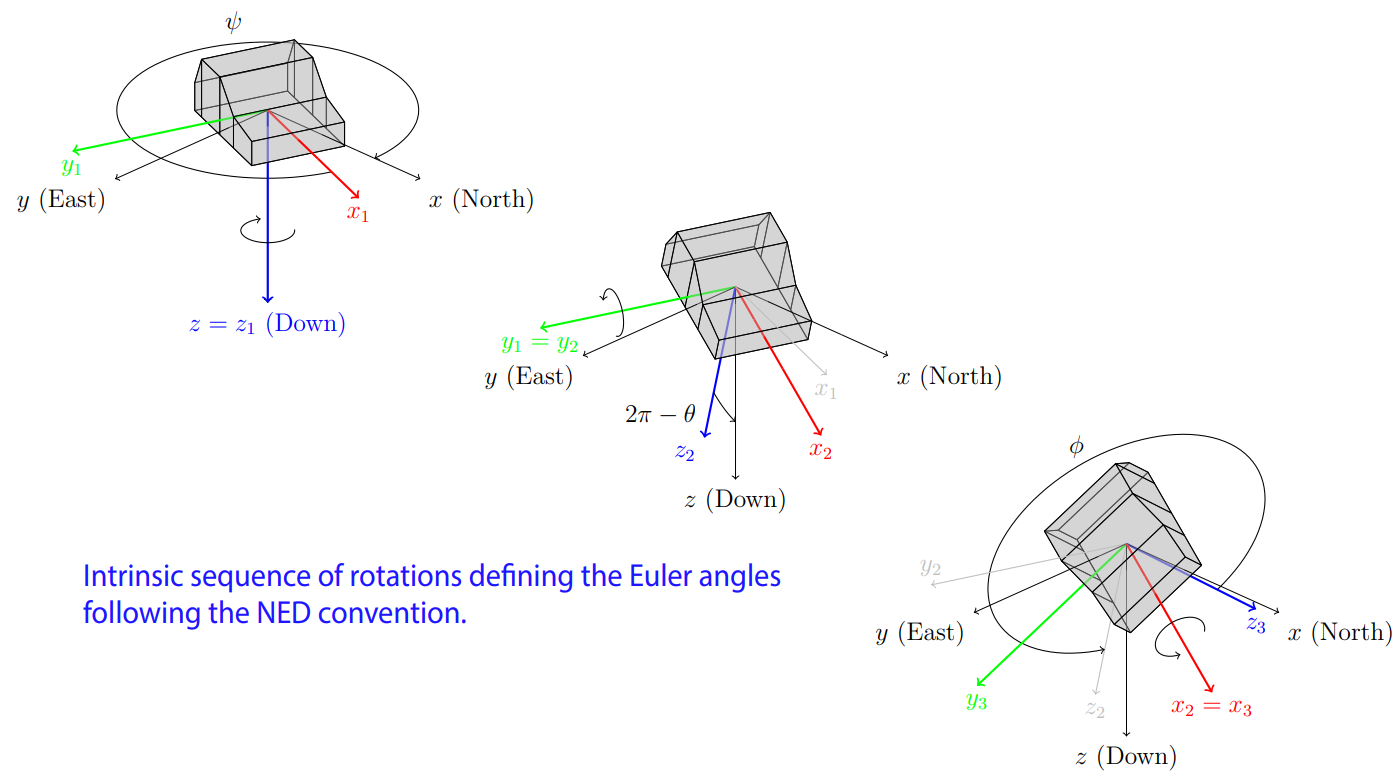
\includegraphics[width=0.9\linewidth]{Pictures/System_Modeling/Orientation_Representations/NED_Frame_EUler_Angles.png}
    \caption{Intrinsic sequence of rotations defining the Euler angles following the NED convention. Figure taken from Edmund Brekke book on Fundamentals of Sensor Fusion.\textsuperscript{\cite{sensor_fusion_book}}}
    \label{fig:system-modeling-ned-euler}
\end{figure}
\noindent
The main advantages of Euler angles are their simplicity, minimal parameter count, and intuitive physical meaning. Each angle directly corresponds to an observable rotational motion, which simplifies both system design and debugging. They also integrate naturally with classical control systems, where angular rates are easily expressed as time derivatives of Euler angles.  
\\ \\
However, the Euler representation suffers from a singularity problem known as \textit{``gimbal lock''}, which in the NED convention occurs when the pitch angle approaches $\theta = \pm90^{\circ}$. At this configuration, the yaw and roll axes align, resulting in the loss of one rotational degree of freedom. In this state, small changes in pitch can cause disproportionately large or undefined changes in yaw and roll rates. Mathematically, the transformation matrix that relates Euler angle rates to body angular velocities becomes ill-conditioned, leading to singularities where the angular rate terms tend toward infinity. This introduces numerical instability and unreliable attitude estimates, which are particularly problematic for navigation and control systems relying on smooth and continuous angular motion.
\\ \\
The relationship between the body angular velocity vector $\boldsymbol{\omega}_b = [p~q~r]^T$ and the Euler angle rate vector $\dot{\boldsymbol{\Theta}} = [\dot{\phi}~\dot{\theta}~\dot{\psi}]^T$ for the NED yaw-pitch-roll convention is expressed as:
$$
    \begin{bmatrix}
        p \\ q \\ r
    \end{bmatrix}
    =
    \begin{bmatrix}
        1 & 0 & -\sin\theta \\
        0 & \cos\phi & \sin\phi\cos\theta \\
        0 & -\sin\phi & \cos\phi\cos\theta
    \end{bmatrix}
    \begin{bmatrix}
        \dot{\phi} \\ \dot{\theta} \\ \dot{\psi}
    \end{bmatrix}
$$
When the pitch angle approaches $\theta = \pm90^{\circ}$, the cosine term $\cos\theta$ tends to zero, causing the matrix to lose rank and become singular. As a result, any attempt to compute Euler rate derivatives or integrate attitude dynamics at this configuration leads to undefined or infinite angular velocities.
\begin{figure}[H]
    \centering
    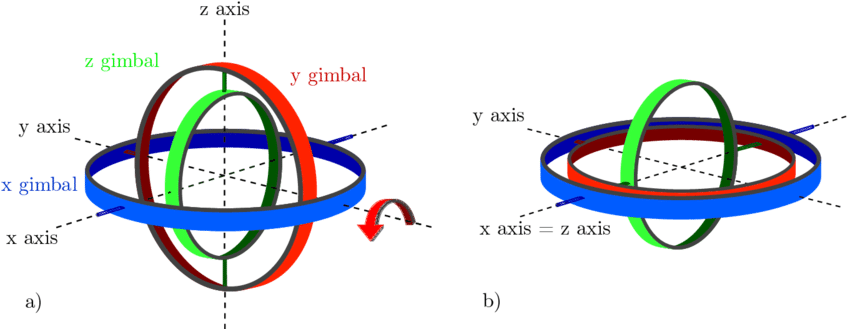
\includegraphics[width=0.9\linewidth]{Pictures/System_Modeling/Orientation_Representations/Gimbal_Lock.png}
    \caption{Illustration of gimbal lock where the yaw and roll axes coincide, causing loss of one rotational degree of freedom. Picture taken from a research paper that explains gimbal lock with illustrations.\textsuperscript{\cite{gimbal_lock}}}
    \label{fig:system-modeling-gimbal-lock}
\end{figure}
\noindent
Despite this limitation, Euler angles remain a practical choice for surface and marine robotics, where pitch and roll angles typically remain small. Their intuitive interpretation and computational simplicity make them well suited for real-time estimation and control near level operating conditions. In the case of an ASV, large attitude excursions are highly unlikely, as excessive roll or pitch would indicate a loss of stability or complete capsizing. Under such operational constraints, the singularity at $\theta = \pm90^{\circ}$ is never encountered, making the Euler representation both sufficient and efficient for navigation and SLAM applications.



\newpage



\subsubsection{Quaternions}
Quaternions provide a compact and singularity free alternative to Euler angles for representing three dimensional orientations. They extend complex numbers into four dimensions and are defined as a scalar and a three component vector
$$
    \mathbf{q} =
    \begin{bmatrix}
        q_w \\ q_x \\ q_y \\ q_z
    \end{bmatrix}
    =
    \begin{bmatrix}
        \cos\frac{\theta}{2} \\
        \hat{u}_x \sin\frac{\theta}{2} \\
        \hat{u}_y \sin\frac{\theta}{2} \\
        \hat{u}_z \sin\frac{\theta}{2}
    \end{bmatrix}
$$
where $\theta$ is the rotation angle and $\hat{u} = [\hat{u}_x~\hat{u}_y~\hat{u}_z]^T$ is the unit vector defining the rotation axis. The quaternion $\mathbf{q}$ therefore represents a rotation of $\theta$ radians about $\hat{u}$. To ensure that it encodes a valid rotation, it must satisfy the unit norm constraint
$$
    \|\mathbf{q}\| = \sqrt{q_w^2 + q_x^2 + q_y^2 + q_z^2} = 1
$$
Normalization is typically enforced after each update step in numerical integration or filtering to avoid drift due to floating point errors. This is done by dividing the quaternion by its magnitude:
$$
    \mathbf{q}_{\text{normalized}} = \frac{\mathbf{q}}{\|\mathbf{q}\|} = 
    \frac{1}{\sqrt{q_w^2 + q_x^2 + q_y^2 + q_z^2}}
    \begin{bmatrix}
        q_w \\ q_x \\ q_y \\ q_z
    \end{bmatrix}
$$
A geometric interpretation of quaternions can be seen in Figure \ref{fig:system-modeling-quaternion-geometry}. Quaternions can be viewed as points on the unit four dimensional hypersphere $S^3$, composed of a real component and a three dimensional imaginary subspace spanned by $(i, j, k)$. The real component represents the cosine of half the rotation angle, while the imaginary vector component encodes the rotation axis scaled by the sine of half the angle. Together, they define a rotation in three dimensional space through the relation $\mathbf{q} = \cos\frac{\theta}{2} + \hat{u}\sin\frac{\theta}{2}$. Each point on this hypersphere corresponds to a unique orientation of a rigid body, and continuous motion along its surface represents a smooth change in attitude without encountering any discontinuities or singularities.  
\\ \\
When a vector $\mathbf{v}$ is rotated using $\mathbf{q}\mathbf{v}\mathbf{q}^{-1}$, the operation effectively applies a double rotation, first through $\mathbf{q}$ and then through its conjugate $\mathbf{q}^{-1}$, producing a single pure 3D rotation about the axis $\hat{u}$ by an angle $\theta$. The scalar part $\cos(\theta/2)$ defines the rotation magnitude, while the vector part $\sin(\theta/2)\hat{u}$ specifies the rotation axis in the imaginary $(i, j, k)$ space. This representation forms the basis for quaternion based attitude kinematics used in estimation and control.
\begin{figure}[H]
    \centering
    \begin{minipage}[b]{0.45\linewidth}
        \centering
        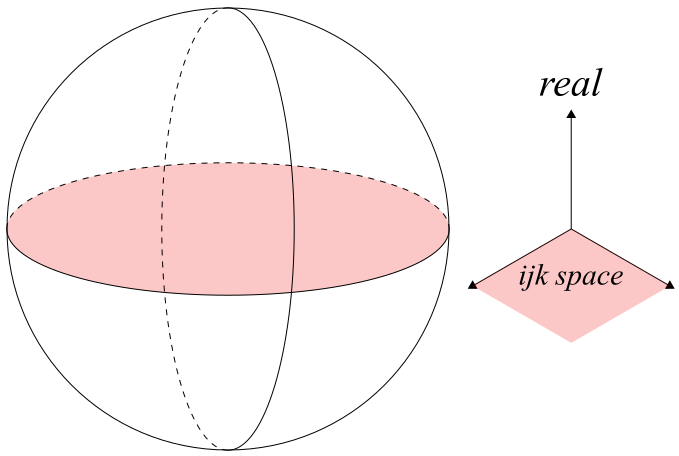
\includegraphics[width=\linewidth]{Pictures/System_Modeling/Orientation_Representations/quaternion_pic1.png}
    \end{minipage}
    \hfill
    \begin{minipage}[b]{0.32\linewidth}
        \centering
        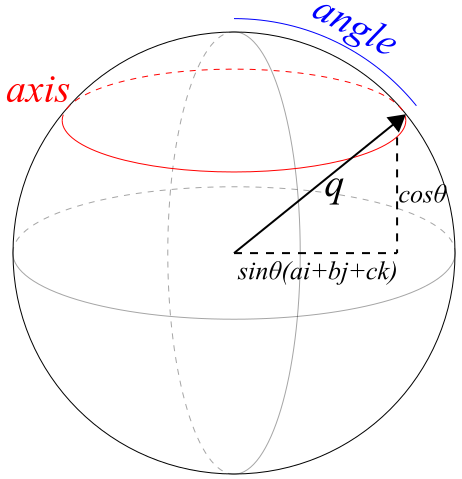
\includegraphics[width=\linewidth]{Pictures/System_Modeling/Orientation_Representations/quaternion_pic2.png}
    \end{minipage}
    \caption{Geometric interpretation of quaternions on the unit hypersphere $S^3$. (Left) Decomposition into the real axis and imaginary $(i, j, k)$ subspace. (Right) Axis-angle representation showing how a quaternion encodes rotation by $\theta$ about the unit axis $\hat{u}$. Picture taken from article that explains quarterion rotation in a intuitive way.\textsuperscript{\cite{quaternions_explained}}}
    \label{fig:system-modeling-quaternion-geometry}
\end{figure}
\noindent
Rotations using quaternions are performed through quaternion multiplication, which is associative but not commutative. Given two orientations $\mathbf{q}_1$ and $\mathbf{q}_2$, their combined rotation is expressed as
$$
    \mathbf{q}_{\text{combined}} = \mathbf{q}_2 \otimes \mathbf{q}_1,
$$
where $\otimes$ denotes the quaternion product. The rotation of a vector $\mathbf{v}$ in three dimensional space can then be performed as
$$
    \mathbf{v}' = \mathbf{q} \otimes \mathbf{v}_q \otimes \mathbf{q}^{-1},
$$
where $\mathbf{v}_q = [0~v_x~v_y~v_z]^T$ is the quaternion form of the vector $\mathbf{v}$. This operation applies the rotation represented by $\mathbf{q}$ to $\mathbf{v}$ in a smooth and continuous manner without encountering singularities.  
\\ \\
For smooth orientation transitions, quaternions can be interpolated using Spherical Linear Interpolation (SLERP). Instead of blending components linearly, SLERP moves along the great circle that connects two orientations on the unit quaternion sphere $S^3$. This ensures that the interpolated motion follows a constant angular velocity and remains at a fixed distance from the sphere center, preserving rotation smoothness and avoiding distortion.  
\\ \\
Given two normalized quaternions $\mathbf{q}_1$ and $\mathbf{q}_2$, the interpolation for $t \in [0,1]$ is defined as
$$
    \text{SLERP}(\mathbf{q}_1, \mathbf{q}_2; t) =
    \frac{\sin((1-t)\Omega)}{\sin(\Omega)}\mathbf{q}_1 +
    \frac{\sin(t\Omega)}{\sin(\Omega)}\mathbf{q}_2,
$$
where $\Omega = \cos^{-1}(\mathbf{q}_1 \cdot \mathbf{q}_2)$ represents the angle between the two quaternions. When $t = 0$, the result is $\mathbf{q}_1$, and when $t = 1$, the result is $\mathbf{q}_2$. Intermediate values of $t$ trace the shortest rotation path between the two orientations.  
\\ \\
This method is widely used in robotics, computer graphics, and navigation to generate smooth transitions between different orientations. SLERP ensures that intermediate orientations are evenly spaced in angular distance, resulting in constant rotational velocity, a property important for stable attitude control and estimation.  
\\ \\
To ensure interpolation follows the shortest possible rotation path, many implementations adjust the sign of one quaternion when their dot product is negative. This avoids interpolation along the long arc (greater than $180^{\circ}$) and guarantees smooth motion along the minimal angular distance. Figure \ref{fig:system-modeling-quaternion-SLERP} illustrates this process, showing both the \textit{``short''} and the \textit{``natural''} interpolation paths along the quaternion sphere.
\begin{figure}[H]
    \centering
    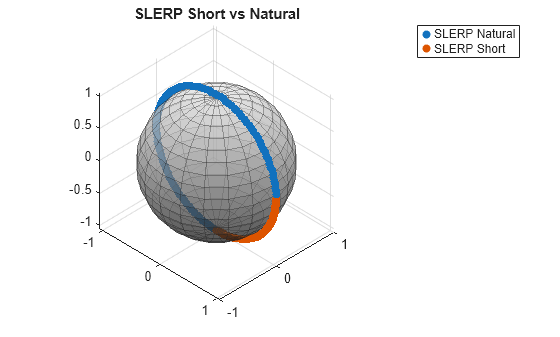
\includegraphics[width=0.75\linewidth]{Pictures/System_Modeling/Orientation_Representations/quaternion_SLERP.png}
    \caption{Spherical linear interpolation (SLERP) between two orientations $\mathbf{q}_1$ and $\mathbf{q}_2$ on the unit quaternion sphere. The \textit{``short''} path minimizes angular distance, while the \textit{``natural''} path follows the original direction without sign correction. Figure taken from MATLAB documentation for illustration purposes.\textsuperscript{\cite{quaternions_SLERP}}}
    \label{fig:system-modeling-quaternion-SLERP}
\end{figure}
\noindent
In practical applications, quaternions are widely used in estimators and sensors where singularity free orientation handling is critical. The IMU on the microAmpere platform outputs attitude in quaternion form, which integrates naturally with sensor fusion algorithms such as the Error State Kalman Filter (ESKF) discussed later in the report. These algorithms rely on quaternion algebra to represent small attitude perturbations efficiently and avoid numerical instability associated with Euler angle singularities.  
\\ \\
The main advantages of quaternions include their smooth and continuous representation of orientation, absence of gimbal lock, and computational efficiency in rotation composition and interpolation. They maintain numerical stability under integration and are well suited for optimization and estimation algorithms. However, quaternions require one additional parameter compared to Euler angles and lack intuitive physical meaning, as their four components do not directly correspond to measurable angular quantities. Furthermore, they are less straightforward to interpret and manipulate mathematically, often requiring specialized operations such as normalization, conjugation, and noncommutative multiplication. Despite these challenges, their robustness and compatibility with modern sensor fusion and control frameworks make quaternions a preferred internal representation for real-time navigation and estimation systems.



\subsubsection{Lie Groups and Manifolds}
Lie groups provide a mathematical framework for representing continuous and smooth transformations such as rotation and translation in three dimensional space. They combine the properties of algebraic groups and differentiable manifolds, allowing both analytical manipulation and geometric interpretation of motion. In navigation, control, and robotics, Lie groups enable consistent handling of orientation and pose without the discontinuities or ambiguities present in minimal representations such as Euler angles.  
\\ \\
The rotation group $\mathrm{SO}(3)$, called the Special Orthogonal Group, represents all possible 3D rotations. Each rotation is described by a $3\times3$ matrix $R$ that satisfies
$$
    R^T R = I, \quad \det(R) = 1
$$
This group is smooth and continuous, meaning that small changes in orientation correspond to small movements on the manifold. To describe small or incremental rotations, $\mathrm{SO}(3)$ is associated with its tangent space, the Lie algebra $\mathfrak{so}(3)$.  
\\ \\
Elements of $\mathfrak{so}(3)$ are skew-symmetric matrices that encode infinitesimal rotations. A rotation vector $\boldsymbol{\omega} = [\omega_x~\omega_y~\omega_z]^T$ can be written as
$$
    \boldsymbol{\omega}^\times =
    \begin{bmatrix}
        0 & -\omega_z & \omega_y \\
        \omega_z & 0 & -\omega_x \\
        -\omega_y & \omega_x & 0
    \end{bmatrix}
$$
This matrix form is simply another way of expressing the cross product $\boldsymbol{\omega} \times \mathbf{v}$, which rotates a vector $\mathbf{v}$ by a small angle.  
\\ \\
The exponential map connects this local representation to an actual finite rotation on $\mathrm{SO}(3)$:
\begin{equation}
    R = \exp(\boldsymbol{\omega}^\times)
    \label{eq:lie-groups-and-manifold-exponential}
\end{equation}
And the inverse operation (the logarithmic map) retrieves the corresponding small rotation from $R$:
\begin{equation}
    \boldsymbol{\omega} = \log(R)
    \label{eq:lie-groups-and-manifold-logarithmic}
\end{equation}
These two functions allow smooth transitions between local angular velocity representations and full 3D orientations, which is highly useful for filters and optimizers for SLAM.  
\\ \\
To include translation as well as rotation, the concept extends to $\mathrm{SE}(3)$, the so called Special Euclidean Group, which describes full 3D rigid body motion:
\begin{equation}
    T =
    \begin{bmatrix}
        R & \mathbf{p} \\
        0 & 1
    \end{bmatrix},
    \quad T \in \mathrm{SE}(3)
    \label{eq:SE3-definition}
\end{equation}
\noindent
Here $R$ is orientation and $\mathbf{p}$ is position. This group provides a consistent mathematical way to represent a vehicles full pose and combine both rotational and translational motion.  
\\ \\
In robotics and navigation, $\mathrm{SO}(3)$ and $\mathrm{SE}(3)$ are used to describe smooth and continuous motion in three dimensional space. $\mathrm{SO}(3)$ represents pure rotations, while $\mathrm{SE}(3)$ extends this to include both rotation and translation, forming the full rigid body pose. These groups define motion directly on the manifold, ensuring mathematically consistent and globally valid transformations without singularities.  
\\ \\
The curved surface of the $\mathrm{SE}(3)$ manifold represents all possible poses of a rigid body in space. The tangent plane at the identity, denoted $\mathfrak{se}(3)$, represents small local motions that can be combined and integrated into full poses using the exponential map $\exp(\cdot)$. Conversely, the logarithmic map $\log(\cdot)$ converts a pose difference back into this local space. Together, these mappings allow smooth transitions between small local displacements and full 3D transformations, which is essential for analyzing and composing motion in robotics and control.  
\\ \\
\begin{figure}[H]
    \centering
    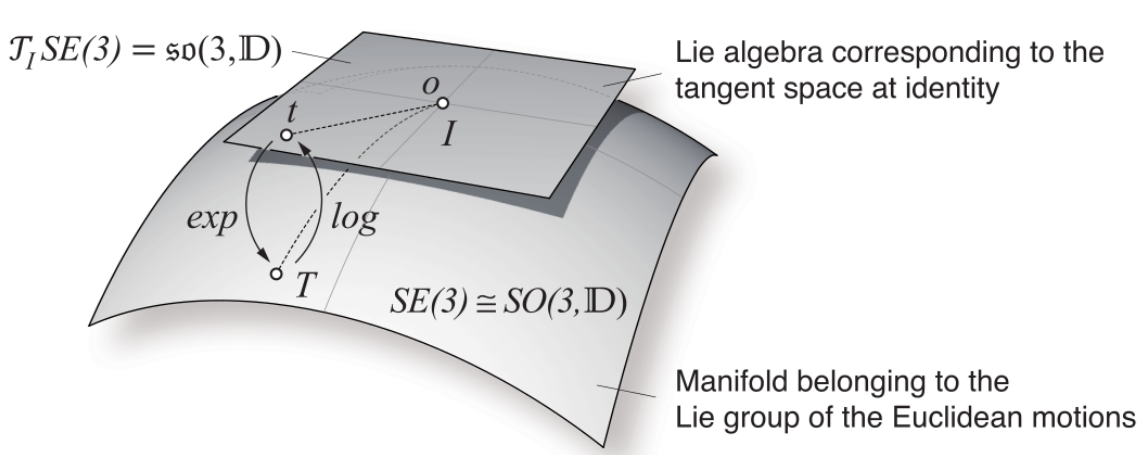
\includegraphics[width=0.8\linewidth]{Pictures/System_Modeling/Orientation_Representations/lie_group_tangent_space.png}
    \caption{Visualization of the $\mathrm{SE}(3)$ manifold and its tangent space $\mathfrak{se}(3)$. Small motions are represented in the tangent space and mapped to the manifold through the exponential map $\exp(\cdot)$, while the logarithmic map $\log(\cdot)$ projects manifold elements back to the local linear space. Figure taken from Nikolay Atanasov lecture notes on Sensing \& Estimation in Robotics.\textsuperscript{\cite{lie_groups_presentation}}}
    \label{fig:system-modeling-so3-se3}
\end{figure}
\noindent
Lie group formulations are fundamental in modern SLAM systems because they provide a mathematically consistent way to represent and manipulate poses in three dimensions. When building and updating a map, each robot or camera pose is an element of $\mathrm{SE}(3)$, combining both rotation and translation into a single compact structure. This allows pose composition, inversion, and differentiation to be performed directly on the manifold without approximations or singularities. In practice, this means that motion updates, sensor transformations, and loop closure corrections can all be handled through clean matrix operations that are both efficient and numerically stable.  
\\ \\
Using Lie groups also enables fast and scalable computation, a necessity when optimizing over thousands of poses and landmarks in large scale SLAM problems. The same mathematical principles are applied in computer graphics and 3D rendering, where $\mathrm{SE}(3)$ transformations are used to efficiently manipulate hundreds or thousands of objects and vertices in real time. By working on the manifold, transformations remain consistent regardless of scale or complexity, ensuring that rotations and translations compose correctly without distortion.  
\\ \\
Overall, Lie group representations allow SLAM and mapping algorithms to combine geometry, motion, and optimization within a single unified framework. They ensure that the estimated trajectory and map remain globally consistent, even after many iterations of motion and correction, making them the foundation of accurate and robust 3D perception in robotics.



\newpage



\subsubsection{Handy Conversions}
The following conversion formulas are taken directly from Edmund Brekkes book on \textit{``Fundamentals of Sensor Fusion''} \cite{sensor_fusion_book}. They are commonly used to convert between different orientation representations for navigation, control, and estimation.
\\ \\
\textbf{Euler to Quaternion}
$$
    \mathbf{q} =
    \begin{bmatrix}
        q_w \\ q_x \\ q_y \\ q_z
    \end{bmatrix}
    =
    \begin{bmatrix}
        \cos\frac{\phi}{2}\cos\frac{\theta}{2}\cos\frac{\psi}{2} + \sin\frac{\phi}{2}\sin\frac{\theta}{2}\sin\frac{\psi}{2} \\
        \sin\frac{\phi}{2}\cos\frac{\theta}{2}\cos\frac{\psi}{2} - \cos\frac{\phi}{2}\sin\frac{\theta}{2}\sin\frac{\psi}{2} \\
        \cos\frac{\phi}{2}\sin\frac{\theta}{2}\cos\frac{\psi}{2} + \sin\frac{\phi}{2}\cos\frac{\theta}{2}\sin\frac{\psi}{2} \\
        \cos\frac{\phi}{2}\cos\frac{\theta}{2}\sin\frac{\psi}{2} - \sin\frac{\phi}{2}\sin\frac{\theta}{2}\cos\frac{\psi}{2}
    \end{bmatrix}
$$
\textbf{Quaternion to Euler}
$$
    \begin{bmatrix}
        \phi \\ \theta \\ \psi
    \end{bmatrix}
    =
    \begin{bmatrix}
        \text{atan2}\big(2(q_w q_x + q_y q_z),\, 1 - 2(q_x^2 + q_y^2)\big) \\
        \text{asin}\big(2(q_w q_y - q_z q_x)\big) \\
        \text{atan2}\big(2(q_w q_z + q_x q_y),\, 1 - 2(q_y^2 + q_z^2)\big)
    \end{bmatrix}
$$
\textbf{Euler to $\mathrm{SO}(3)$}
$$
    R_{from}^{to} = R_{b}^{n} = R_x(\phi) R_y(\theta) R_z(\psi)
$$
$$
    R_x(\phi) =
    \begin{bmatrix}
        1 & 0 & 0 \\
        0 & \cos\phi & -\sin\phi \\
        0 & \sin\phi & \cos\phi
    \end{bmatrix}, \quad
    R_y(\theta) =
    \begin{bmatrix}
        \cos\theta & 0 & \sin\theta \\
        0 & 1 & 0 \\
        -\sin\theta & 0 & \cos\theta
    \end{bmatrix}, \quad
    R_z(\psi) =
    \begin{bmatrix}
        \cos\psi & -\sin\psi & 0 \\
        \sin\psi & \cos\psi & 0 \\
        0 & 0 & 1
    \end{bmatrix}
$$
\textbf{Quaternion to $\mathrm{SO}(3)$}
$$
    R_{from}^{to} = R_{b}^{n} =
    \begin{bmatrix}
        1 - 2(q_y^2 + q_z^2) & 2(q_x q_y - q_z q_w) & 2(q_x q_z + q_y q_w) \\
        2(q_x q_y + q_z q_w) & 1 - 2(q_x^2 + q_z^2) & 2(q_y q_z - q_x q_w) \\
        2(q_x q_z - q_y q_w) & 2(q_y q_z + q_x q_w) & 1 - 2(q_x^2 + q_y^2)
    \end{bmatrix}
$$
\\ \\
\noindent
These relationships provide a convenient reference for converting between orientation representations depending on the application, whether for computation, visualization, or integration with sensor data.
 \clearpage
\subsection{Reference Frames and Transformations}
\subsubsection{Basic Translation and Rotation Transformations}
Rigid body motion in three dimensions can be expressed compactly using the homogeneous transformation matrix $T \in \mathrm{SE}(3)$ defined in Equation \ref{eq:SE3-definition}. These matrices combine rotation and translation into a single representation and are used to map coordinates between frames such as the navigation (NED), body, and sensor frames.  
\\ \\
The pose of the body frame relative to the navigation frame is written as
$$
    T_{b}^{n} =
    \begin{bmatrix}
        R_{b}^{n} & \mathbf{p}_{b}^{n} \\
        0 & 1
    \end{bmatrix}
$$
where $R_{b}^{n}$ is the rotation matrix from the body to the NED frame, and $\mathbf{p}_{b}^{n}$ is the position of the body origin expressed in NED coordinates.
\\ \\
A point $\mathbf{x}_{b}^{b}$ expressed in the body frame can be transformed to the NED frame as:
$$
    \mathbf{x}_{b}^{n}=
    T_{b}^{n}
    \begin{bmatrix}
        \mathbf{x}_{b}^{b} \\ 1
    \end{bmatrix}
    = R_{b}^{n}\mathbf{x}_{b}^{b} + \mathbf{p}_{b}^{n}
$$
\noindent
Composing multiple transformations is performed through matrix multiplication. For instance, if $T_{s}^{b}$ defines the transformation from a sensor frame to the body frame, then the sensor pose in the NED frame becomes
$$
    T_{s}^{n} = T_{b}^{n} T_{s}^{b}
$$
The inverse transformation, which converts coordinates from NED back to the body frame, is given by
$$
    T_{n}^{b} = (T_{b}^{n})^{-1} =
    \begin{bmatrix}
        (R_{b}^{n})^T & -(R_{b}^{n})^T \mathbf{p}_{b}^{n} \\
        0 & 1
    \end{bmatrix}
$$
This matrix formulation provides a clean and consistent way to represent spatial relationships between the navigation, body, and sensor frames. It is fundamental in robotics, navigation, and control, where accurate frame alignment and transformation chaining are essential for pose estimation and sensor fusion.
\\ \\
These homogeneous transformations form the foundation for defining global and local reference frames such as WGS84, ECEF, NED, and Body, which are described in the following sections



\subsubsection{Global Reference Frames}
Global reference frames provide the foundation for representing absolute positions on Earth and are essential for all GNSS based navigation and mapping systems. Since GNSS receivers provide position estimates in a global Earth fixed frame, while navigation and control systems typically operate in local frames such as NED or body coordinates, it becomes necessary to define consistent global reference models to enable accurate transformations between these coordinate systems.   
\\ \\
The two main reference systems used for this purpose are the World Geodetic System 1984 (WGS84) geodetic model, which defines the Earths ellipsoidal shape and geodetic coordinates (latitude, longitude, altitude), and the Earth-Centered Earth-Fixed (ECEF) Cartesian frame, which expresses these same positions as 3D Cartesian coordinates centered at the Earths center of mass. These systems provide the common link between GNSS measurements and local navigation frames used in estimation and control.
\\ \\
\textbf{WGS84} 
\\ \noindent
The World Geodetic System 1984 (WGS84) is the global geodetic reference used by all major GNSS systems. It defines an Earth-fixed ellipsoidal model that closely approximates the planets mean shape, accounting for the equatorial bulge caused by rotation. Although regional realizations such as \textit{``ETRS89''} (European Terrestrial Reference System 1989) are used in Europe to reduce tectonic drift, the WGS84 reference remains the standard for GNSS based navigation in Norway and most marine applications, with differences between the two systems being only a few decimeters.
\\ \\
The WGS84 model defines the Earth as an oblate ellipsoid, flattened at the poles and expanded at the equator. It serves as the global geodetic reference for GPS and most modern satellite navigation systems. The ellipsoid parameters are defined as $a = 6378137.0~\text{m}$ and $f = 1/298.257223563$, where $a$ is the semi major axis and $f$ is the flattening factor. The semi minor axis can then be computed as $b = a(1-f)$.  
\\ \\
A position on Earth is defined by three geodetic coordinates. First the latitude $\varphi$, which is the angle between the equatorial plane and the ellipsoid normal. Then the longitude $\lambda$, which is the angle between the Greenwich meridian and the projection of the point onto the equatorial plane. Finally the altitude $h$, which is the height above the ellipsoidal surface. These coordinates describe a points global position and are the standard output format from all GNSS receivers.
\begin{figure}[H]
    \centering
    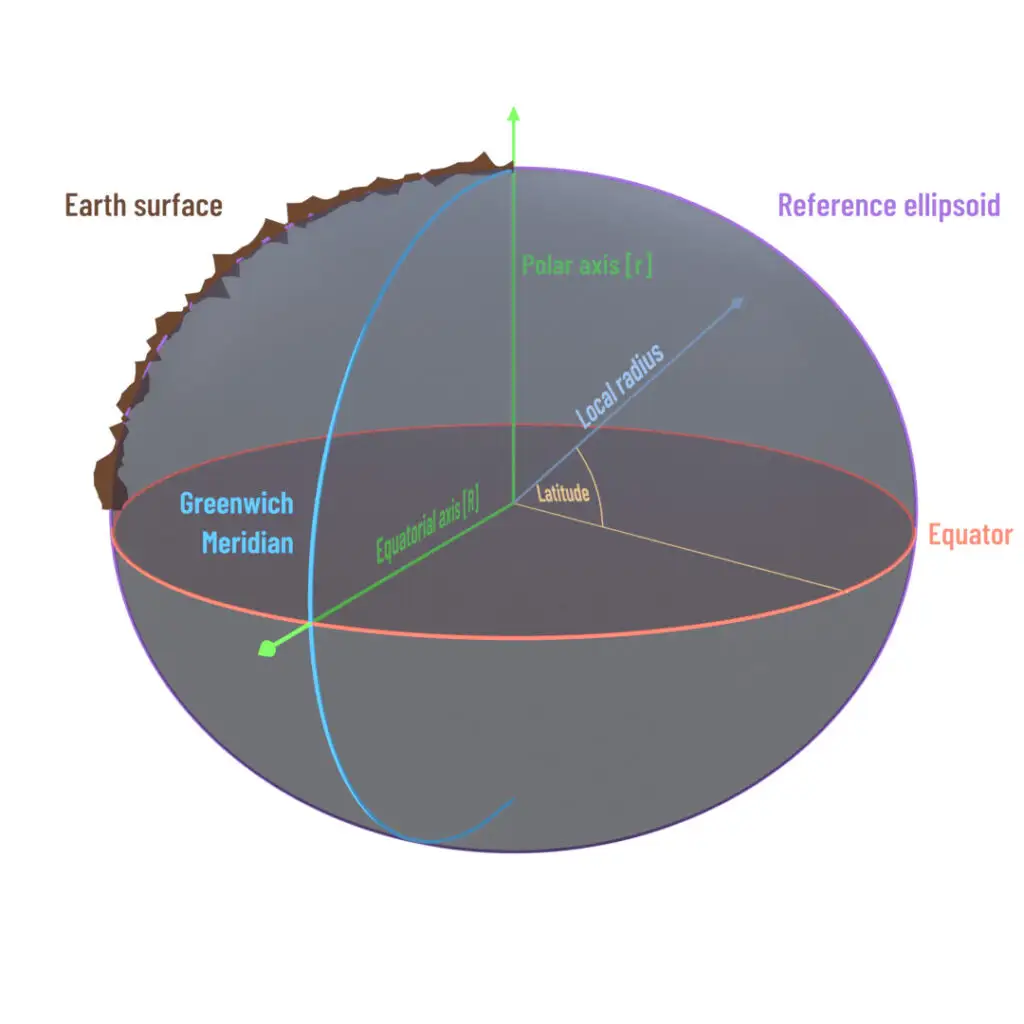
\includegraphics[width=0.7\linewidth]{Pictures/System_Modeling/Reference_Frames_and_Transformations/WGS84.png}
    \caption{WGS84 ellipsoidal Earth model showing the relationship between latitude, longitude, and altitude. Figure taken from GeneSys Elektronik GmbH documentation.\textsuperscript{\cite{WGS84}}}
    \label{fig:system-Modeling-wgs84-ellipsoid}
\end{figure}
\noindent
\textbf{ECEF}
\\ \noindent
The Earth-Centered Earth-Fixed (ECEF) frame is a three dimensional Cartesian coordinate system with its origin at the Earths center of mass. The $x$-axis passes through the intersection of the equator and the Greenwich meridian, the $y$-axis lies along the equator $90^{\circ}$ east of the $x$-axis, and the $z$-axis points toward the North Pole. The ECEF frame rotates with the Earth and is commonly used for expressing GNSS positions in Cartesian form.  
\\ \\
The transformation from geodetic coordinates WGS84 $(\varphi, \lambda, h)$ to ECEF coordinates $(x, y, z)$ is given by:
$$
    \begin{aligned}
        e^2 &= 2f - f^2, \\
        N(\varphi) &= \frac{a}{\sqrt{1 - e^2 \sin^2\varphi}}, \\
        x &= (N(\varphi) + h)\cos\varphi\cos\lambda, \\
        y &= (N(\varphi) + h)\cos\varphi\sin\lambda, \\
        z &= \big[(1 - e^2)N(\varphi) + h\big]\sin\varphi
    \end{aligned}
$$
where $N(\varphi)$ is the prime vertical radius of curvature and $e$ is the first eccentricity of the ellipsoid. The inverse conversion from ECEF to geodetic coordinates is typically solved iteratively due to the nonlinear nature of the equations.
\begin{figure}[H]
    \centering
    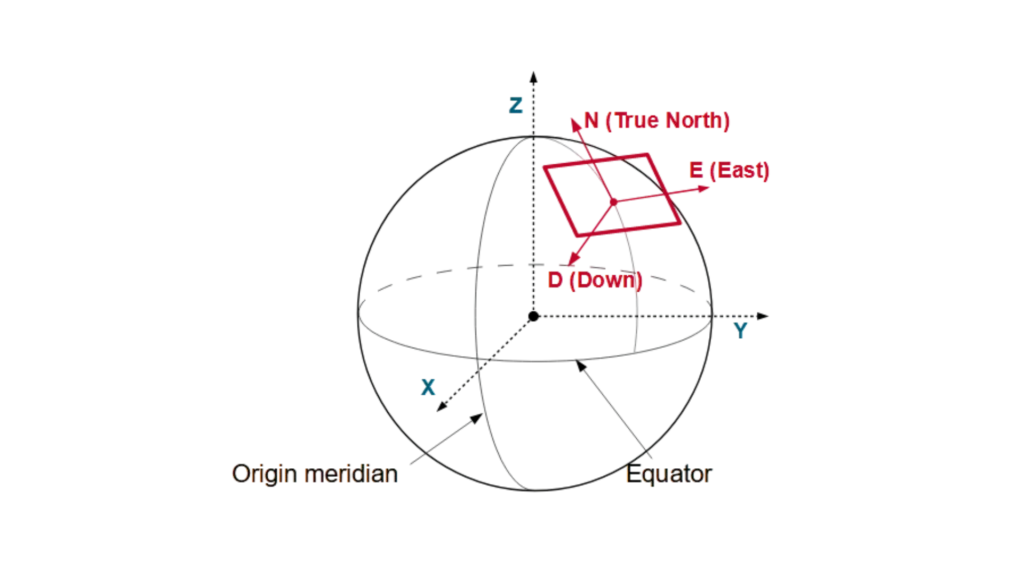
\includegraphics[width=0.9\linewidth]{Pictures/System_Modeling/Reference_Frames_and_Transformations/ECEF.png}
    \caption{Earth-Centered Earth-Fixed (ECEF) coordinate system with origin at Earth's center and axes aligned with the equator and rotational axis. Figure taken from open source GNSS reference material.\textsuperscript{\cite{ECEF}}}
    \label{fig:ecef-frame}
\end{figure}
\noindent
The WGS84 and ECEF frames together form the foundation of all global navigation and positioning systems. While WGS84 defines the geometric reference ellipsoid used by GNSS measurements, ECEF provides a Cartesian coordinate representation that is better suited for numerical computation, sensor fusion, and integration with local navigation frames such as NED or body fixed coordinates.



\subsubsection{Local Reference Frames}
Local reference frames are used to describe the motion and orientation of vehicles in a way that is intuitive and convenient for navigation, estimation, and control. In marine and aerial systems, the two most common local frames are the North-East-Down (NED) frame and the Body frame. These provide a consistent way to represent vehicle states such as position, velocity, and attitude relative to the Earth.  
\\ \\
The NED frame is a local tangent frame fixed to a point on the Earths surface, with the $x$-axis pointing toward geographic north, the $y$-axis pointing east, and the $z$-axis pointing downward, perpendicular to the ellipsoid. This convention is widely used in navigation because it aligns naturally with compass directions and simplifies interpretation of GNSS and IMU data. The origin of the NED frame is typically defined at a reference point near the vehicles initial position, tangent to the Earth at that location.  
\\ \\
The Body frame is attached to the vehicle itself, with its origin at the vehicles center of gravity or another defined point. The $x$-axis points forward along the vehicles longitudinal direction, the $y$-axis points to the right, and the $z$-axis points downward. All onboard sensor measurements, such as accelerations, angular velocities, and forces, are naturally expressed in this frame.  
\\ \\
\begin{figure}[H]
    \centering
    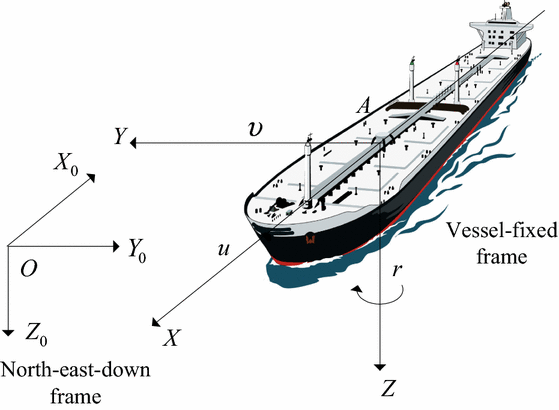
\includegraphics[width=0.55\linewidth]{Pictures/System_Modeling/Reference_Frames_and_Transformations/NED.png}
    \caption{NED coordinate system attached to a marine vehicle. The illustration shows the local navigation axes and their relation to the body frame. Figure taken from a report on robust nonlinear control design for dynamic positioning of marine vessels.\textsuperscript{\cite{NED}}}
    \label{fig:system-modeling-ned-frame}
\end{figure}
\noindent
The relationship between the global and local reference frames follows the transformation chain:
$$
    \text{WGS84 (geodetic)} \;\rightarrow\; \text{ECEF (Cartesian)} \;\rightarrow\; \text{NED (local tangent)} \;\rightarrow\; \text{Body (vehicle-fixed)}
$$
GNSS receivers typically provide positions in the WGS84 frame, expressed as geodetic coordinates $(\varphi, \lambda, h)$, where $\varphi$ is latitude, $\lambda$ is longitude, and $h$ is altitude above the reference ellipsoid. For computational purposes, these coordinates are first converted to the ECEF frame, which represents positions in Cartesian coordinates $(x, y, z)$ relative to the Earth's center of mass.  
\\ \\
To obtain a local navigation frame, the ECEF position is then rotated and translated into the NED frame, which defines a tangent plane fixed at a chosen reference point $(\varphi_0, \lambda_0)$. The rotation from ECEF to NED is given by
$$
    R_{e}^{n} =
    \begin{bmatrix}
        -\sin\varphi_0\cos\lambda_0 & -\sin\varphi_0\sin\lambda_0 & \cos\varphi_0 \\
        -\sin\lambda_0 & \cos\lambda_0 & 0 \\
        -\cos\varphi_0\cos\lambda_0 & -\cos\varphi_0\sin\lambda_0 & -\sin\varphi_0
    \end{bmatrix}
$$
where $\varphi_0$ and $\lambda_0$ are the latitude and longitude of the local origin. The superscript $n$ and subscript $e$ indicate that this matrix transforms a vector expressed in the ECEF frame $\{e\}$ into the NED frame $\{n\}$.  
\\ \\
Given the ECEF position of the vehicle $\mathbf{p}_{b/e}^{e}$ and the ECEF position of the NED origin $\mathbf{p}_{O/e}^{e}$, the vehicles position in NED coordinates is computed as
$$
    \mathbf{p}_{b/O}^{n} = \mathbf{p}_{b/e}^{n} + \mathbf{p}_{e/O}^{n} = R_e^n (\mathbf{p}_{b/e}^{e} - \mathbf{p}_{O/e}^{e})
$$
For onboard sensors, the position of a sensor $\{s\}$ relative to the vehicle body origin, expressed in the NED frame, is given by
$$
\mathbf{p}_{s/b}^{n} = R_b^n \mathbf{p}_{s/b}^{b}
$$
The absolute position of the sensor relative to the NED origin can then be found as
$$
\mathbf{p}_{s/O}^{n} = \mathbf{p}_{s/b}^{n} + \mathbf{p}_{b/O}^{n}
$$
where $\mathbf{p}_{s/b}^{b}$ is the known position of the sensor in the body frame, and $R_b^n$ is the rotation matrix representing the vehicles attitude from the Body to the NED frame.
\\ \\
This formulation relates the sensor position to the global reference frame by first rotating the sensor offset from the body frame into the navigation frame, then translating it using the vehicles global position. The rotation matrix $R_b^n$ is obtained from the vehicles orientation representation, typically parameterized using Euler angles or a unit quaternion, ensuring consistent alignment between the sensor, body, and navigation coordinate frames.
\\ \\
Maintaining a consistent chain of transformations between these frames is essential for reliable navigation and estimation. In practice, GNSS delivers global positions in WGS84 or ECEF coordinates, while onboard IMU sensors provide measurements in the Body frame. Sensor fusion algorithms such as the Extended Kalman Filter (EKF) and Error State Kalman Filter (ESKF) depend on these transformations to express all quantities consistently within the NED frame used for state estimation and control.
 \clearpage
\subsection{Rigid Body Kinematics}
\subsubsection{Relevance for Navigation and Modeling}
Rigid body kinematics provides the mathematical foundation for expressing motion, orientation, and acceleration consistently across coordinate frames. In navigation systems, these relationships allow the integration of measurements from inertial sensors, GNSS, and other sources within a unified dynamic model.  
\\ \\
The transformation equations for position, velocity, and acceleration ensure that sensor data expressed in the body frame can be accurately related to the navigation frame, enabling correct estimation of the vehicles state. This consistency is essential for inertial navigation, attitude estimation, and sensor fusion, where body fixed measurements such as angular velocity and specific force must be mapped into global coordinates for integration and correction.  
\\ \\
Moreover, the rigid body framework is fundamental for simulation and control system design. It allows modeling of vehicle dynamics, actuator response, and sensor placement with precise spatial relationships. The kinematic expressions derived in this section thus serve as the basis for dynamic modeling, state estimation, and motion prediction used in autonomous and navigation systems.



\subsubsection{Position and Orientation}
The position of a rigid body is represented by the vector $\mathbf{p}_{b/O}^{n}$, which denotes the location of the body frame origin expressed in the navigation (NED) frame. The orientation of the body is represented by the rotation matrix $R_b^n \in \mathrm{SO}(3)$, which maps a vector from the body frame $\{b\}$ to the navigation frame $\{n\}$.  
\\ \\
The combined rigid body pose is described by the homogeneous transformation matrix $T_{b/O}^{n} \in \mathrm{SE}(3)$:
$$
    T_{b/O}^{n} =
    \begin{bmatrix}
        R_b^n & \mathbf{p}_{b/O}^{n} \\
        0 & 1
    \end{bmatrix}
$$
The kinematic relationship between the time derivative of position and the linear velocity is then given by
$$
    \dot{\mathbf{p}}_{b/O}^{n} = \mathbf{v}_{b/O}^{n}
$$
where $\mathbf{v}_{b/O}^{n}$ is the velocity of the body origin expressed in the navigation frame.  



\subsubsection{Angular Velocity and Euler Angle Relationship}
The angular velocity vector $\boldsymbol{\omega}_{b/O}^{b} = [p, q, r]^\top$ represents the instantaneous rotation rate of the body about its own axes, roll rate $p$ about the $x_b$-axis (North), pitch rate $q$ about the $y_b$-axis (East), and yaw rate $r$ about the $z_b$-axis (Down).  
\\ \\
When the body orientation is represented by ZYX Euler angles (yaw $\psi$, pitch $\theta$, roll $\phi$), the time derivative of the Euler angles relates to the body angular velocity through
$$
    \begin{bmatrix}
        \dot{\phi} \\ \dot{\theta} \\ \dot{\psi}
    \end{bmatrix}
    = T(\phi, \theta)\boldsymbol{\omega}_{b/O}^{b}
$$
where the transformation matrix $T(\phi, \theta)$ for the NED convention is defined as
$$
    T(\phi, \theta) =
    \begin{bmatrix}
        1 & \sin\phi\tan\theta & \cos\phi\tan\theta \\
        0 & \cos\phi & -\sin\phi \\
        0 & \sin\phi/\cos\theta & \cos\phi/\cos\theta
    \end{bmatrix}
$$
This maps the body angular velocity to the Euler angle rates according to the NED convention.  
\\ \\
The inverse relationship, expressing body angular velocity from Euler angle derivatives, is given by
$$
    \boldsymbol{\omega}_{b/O}^{b} =
    \begin{bmatrix}
        p \\ q \\ r
    \end{bmatrix}
    = T^{-1}(\phi, \theta)
    \begin{bmatrix}
        \dot{\phi} \\ \dot{\theta} \\ \dot{\psi}
    \end{bmatrix}
$$
where
$$
    T^{-1}(\phi, \theta) =
    \begin{bmatrix}
        1 & 0 & -\sin\theta \\
        0 & \cos\phi & \sin\phi\cos\theta \\
        0 & -\sin\phi & \cos\phi\cos\theta
    \end{bmatrix}
$$
This formulation aligns with the NED coordinate convention and ensures correct mapping between angular velocities and Euler angle derivatives. The transformation matrix becomes singular at $\theta = \pm 90^\circ$, corresponding to gimbal lock, where $\tan\theta$ diverges.  



\subsubsection{Angular Velocity and Quaternion Relationship}
Quaternions provide a compact and singularity free representation of rotation. A unit quaternion $q = [q_0, q_1, q_2, q_3]^\top$ consists of one scalar and three vector components, often written as
$$
    q = 
    \begin{bmatrix}
        q_0 \\ \mathbf{q}_v
    \end{bmatrix}
    =
    \begin{bmatrix}
        q_0 \\ q_1 \\ q_2 \\ q_3
    \end{bmatrix}
$$
where $q_0$ is the scalar part and $\mathbf{q}_v = [q_1, q_2, q_3]^\top$ is the vector part.  
The quaternion represents a rotation of angle $\theta$ around the unit axis $\hat{\mathbf{u}}$:
$$
    q =
    \begin{bmatrix}
        \cos\frac{\theta}{2} \\ \hat{\mathbf{u}}\sin\frac{\theta}{2}
    \end{bmatrix}
$$
The time evolution of the quaternion is governed by the angular velocity vector $\boldsymbol{\omega}_{b/O}^{b} = [p, q, r]^\top$ measured in the body frame. The quaternion kinematics are given by
$$
    \dot{q} = \frac{1}{2}\Omega(\boldsymbol{\omega}_{b/O}^{b}) q
$$
where $\Omega(\boldsymbol{\omega}_{b/O}^{b})$ is the quaternion rate matrix:
$$
    \Omega(\boldsymbol{\omega}_{b/O}^{b}) =
    \begin{bmatrix}
        0 & -p & -q & -r \\
        p & 0 & r & -q \\
        q & -r & 0 & p \\
        r & q & -p & 0
    \end{bmatrix}
$$
Given the quaternion $q = [q_0, \mathbf{q}_v]^\top$ and its time derivative $\dot{q} = [\dot{q_0}, \dot{\mathbf{q}_v}]^\top$, the body angular velocity can be reconstructed directly as
$$
    \boldsymbol{\omega}_{b/O}^{b} = 2 \big( q_0\dot{\mathbf{q}_v} - \dot{q_0}\mathbf{\mathbf{q}_v} - \mathbf{\mathbf{q}_v}^{\times}\dot{\mathbf{q}_v} \big).
$$
Here, $q_0$ is the scalar part of the quaternion and $\mathbf{q}*v$ its vector part. This relation provides a direct and numerically stable way to compute the instantaneous angular velocity from quaternion derivatives while maintaining full consistency with rigid body rotational kinematics in the body frame. This formulation complements the quaternion rate equation which integrates angular velocity to update attitude over time. The quaternion must remain normalized, i.e. $|q| = 1$, to represent a valid rotation, and is therefore periodically renormalized during numerical integration as
$$
q = \frac{q}{|q|}.
$$
The corresponding rotation matrix from body to navigation frame is obtained as
$$
    R_b^n(q) =
    \begin{bmatrix}
        1 - 2(q_2^2 + q_3^2) & 2(q_1 q_2 - q_0 q_3) & 2(q_1 q_3 + q_0 q_2) \\
        2(q_1 q_2 + q_0 q_3) & 1 - 2(q_1^2 + q_3^2) & 2(q_2 q_3 - q_0 q_1) \\
        2(q_1 q_3 - q_0 q_2) & 2(q_2 q_3 + q_0 q_1) & 1 - 2(q_1^2 + q_2^2)
    \end{bmatrix}
$$
This rotation matrix provides the mapping between the body and navigation frames, analogous to $R_b^n$ obtained from Euler angles, but without the gimbal lock problem.  
\\ \\
In practice, quaternion based orientation integration using $\dot{q} = \frac{1}{2}\Omega(\boldsymbol{\omega}_{b/O}^{b})q$ is preferred for real-time attitude propagation, while the equivalent rotation matrix or Euler angles are extracted only when needed for visualization or control.



\subsubsection{Linear Velocity Relationship}
The linear velocity of any point $P$ fixed on a rigid body can be related to the velocity of a reference point $O$ on the same body as
$$
    \mathbf{v}_{P/O}^{b} = \mathbf{v}_{b/O}^{b} + \mathbf{v}_{P/b}^{b} + \boldsymbol{\omega}_{b/O}^{b} \times \mathbf{p}_{P/b}^{b}
$$
Here, $\mathbf{v}_{b/O}^{b}$ is the translational velocity of the body origin expressed in the body frame, $\mathbf{v}_{P/b}^{b}$ is the velocity of point $P$ relative to the body (zero for fixed sensors), $\boldsymbol{\omega}_{b/O}^{b}$ is the body angular velocity, and $\mathbf{p}_{P/b}^{b}$ is the position of $P$ relative to the body origin, both expressed in the body frame.
\\ \\
The cross product term $\boldsymbol{\omega}_{b/O}^{b} \times \mathbf{p}_{P/b}^{b}$ represents the additional linear velocity experienced by point $P$ due to the rotational motion of the body. This term becomes more significant for points located farther away from the rotation axis, such as antennas or sensors mounted away from the vessels center of gravity.
\\ \\
In many applications, it is necessary to express all velocities in a common reference frame. The velocity of the body origin expressed in the navigation (NED) frame is obtained by rotating the body frame velocity using the rotation matrix $R_b^n$:
$$
    \mathbf{v}_{b/O}^{n} = R_b^n \mathbf{v}_{b/O}^{b}.
$$
Conversely, the body frame velocity can be obtained from the navigation frame velocity by
$$
    \mathbf{v}_{b/O}^{b} = (R_b^n)^\top \mathbf{v}_{b/O}^{n},
$$
since $(R_b^n)^\top = R_n^b$. The rotation matrix $R_b^n$ is derived from the vehicles orientation, represented either by Euler angles or a unit quaternion.
\\ \\
Similarly, for a sensor or point $P$ rigidly fixed to the vehicle (i.e., $\mathbf{v}_{P/b}^{b} = 0$), the velocity expressed in the navigation frame simplifies to
$$
 \mathbf{v}_{P/O}^{n} = R_b^n \left(\mathbf{v}_{b/O}^{b} + \boldsymbol{\omega}_{b/O}^{b} \times \mathbf{p}_{P/b}^{b}\right),
$$
where $\mathbf{p}_{P/b}^{b}$ defines the sensors position in the body frame. This formulation provides a consistent way to compute the motion of any fixed point on the vehicle in both body and navigation frames, ensuring proper alignment between inertial and navigation states.



\subsubsection{Angular Acceleration in Euler Representation}
The angular acceleration $\boldsymbol{\alpha}_{b/O}^{b}$ describes the rate of change of the body's angular velocity vector $\boldsymbol{\omega}_{b/O}^{b} = [p, q, r]^\top$, which represents the instantaneous rotation of the body about its own $x$, $y$, and $z$ axes. Physically, $\boldsymbol{\alpha}_{b/O}^{b}$ captures how fast the rotational motion itself is changing, and it directly relates to the torques acting on the body through the rotational dynamics equations.  
\\ \\
When the body orientation is represented using Euler angles $(\phi, \theta, \psi)$, the angular acceleration can be obtained by differentiating the Euler angle to angular velocity relationship:
$$
    \boldsymbol{\alpha}_{b/O}^{b} = T^{-1}(\phi, \theta, \psi)\ddot{\boldsymbol{\Theta}} + \dot{T}^{-1}(\phi, \theta, \psi)\dot{\boldsymbol{\Theta}}
$$
where $\dot{\boldsymbol{\Theta}} = [\dot{\phi}, \dot{\theta}, \dot{\psi}]^\top$ and $\ddot{\boldsymbol{\Theta}} = [\ddot{\phi}, \ddot{\theta}, \ddot{\psi}]^\top$ are the first and second derivatives of the Euler angles. The first term represents the direct contribution from angular rate changes, while the second term captures coupling effects caused by the nonlinearity of rotational kinematics, for instance, when pitch or roll rates influence yaw acceleration.  
\\ \\
In differential form, the time derivative of angular velocity is expressed as
$$
    \dot{\boldsymbol{\omega}}_{b/O}^{b} = \boldsymbol{\alpha}_{b/O}^{b}
$$
which defines angular acceleration in the same frame as $\boldsymbol{\omega}_{b/O}^{b}$. To express angular acceleration in another reference frame, such as the navigation frame, it can be transformed using the rotation matrix:
$$
    \boldsymbol{\alpha}_{b/O}^{n} = R_b^n \boldsymbol{\alpha}_{b/O}^{b}
$$
where $R_b^n$ is the rotation from the body frame to the navigation (NED) frame.  
\\ \\
In practical navigation and control systems, the angular acceleration $\boldsymbol{\alpha}_{b/O}^{b}$ is rarely measured directly. It is usually approximated by differentiating the body angular velocity $\boldsymbol{\omega}_{b/O}^{b}$ obtained from gyroscopes or inferred from rigid body dynamics. Maintaining consistent frame alignment between body and navigation frames is essential for accurate attitude propagation and torque computation.



\subsubsection{Angular Acceleration in Quaternion Representation}
The quaternion representation provides a singularity free alternative to Euler angles for describing rotational motion. The unit quaternion $q = [q_0, q_1, q_2, q_3]^\top$ defines the orientation of the body frame relative to the navigation frame, where $q_0$ is the scalar part and $[q_1, q_2, q_3]^\top$ is the vector part.  
\\ \\
The time evolution of the quaternion is governed by the rotational kinematics equation:
$$
    \dot{q} = \frac{1}{2}\Omega(\boldsymbol{\omega}_{b/O}^{b})q
$$
where $\boldsymbol{\omega}_{b/O}^{b} = [p, q, r]^\top$ is the angular velocity in the body frame and $\Omega(\boldsymbol{\omega}_{b/O}^{b})$ is the quaternion rate matrix:
$$
    \Omega(\boldsymbol{\omega}_{b/O}^{b}) =
    \begin{bmatrix}
        0 & -p & -q & -r \\
        p &  0 &  r & -q \\
        q & -r &  0 &  p \\
        r &  q & -p &  0
    \end{bmatrix}
$$
Differentiating this expression gives the quaternion based angular acceleration:
$$
    \ddot{q} = \frac{1}{2}\Omega(\boldsymbol{\alpha}_{b/O}^{b})q + \frac{1}{2}\Omega(\boldsymbol{\omega}_{b/O}^{b})\dot{q}
$$
which captures both the direct contribution of angular acceleration $\boldsymbol{\alpha}_{b/O}^{b}$ and the coupling effect from the current angular velocity.  
\\ \\
In vector form, the time derivative of angular velocity is expressed as
$$
    \dot{\boldsymbol{\omega}}_{b/O}^{b} = \boldsymbol{\alpha}_{b/O}^{b}
$$
which defines angular acceleration in the same frame as $\boldsymbol{\omega}^b$. To express angular acceleration in another reference frame, such as the navigation frame, it can be transformed using the rotation matrix:
$$
    \boldsymbol{\alpha}_{b/O}^{n} = R_b^n \boldsymbol{\alpha}_{b/O}^{b}
$$
where $R_b^n$ is the rotation matrix from body to navigation frame.
\\ \\
To ensure $q$ remains a valid rotation, it must satisfy the unit norm constraint:
$$
    \|q\| = 1
$$
which is typically enforced by periodic normalization during numerical integration like so:
$$
    q = \frac{q}{\|q\|}
$$  
This quaternion based formulation is computationally efficient and avoids the gimbal lock issue inherent in Euler angle representations. For this reason, quaternion propagation is widely preferred for representing orientation and modeling angular dynamics in navigation and control systems.



\subsubsection{Linear Acceleration}
The linear acceleration of a point $P$ on a rigid body consists of translational, tangential, centripetal, and Coriolis components. It is expressed in the body frame as
$$
    \mathbf{a}_{P/O}^{b} =
    \mathbf{a}_{b/O}^{b}
    + \mathbf{a}_{P/b}^{b}
    + \boldsymbol{\alpha}_{b/O}^{b} \times \mathbf{p}_{P/b}^{b}
    + \boldsymbol{\omega}_{b/O}^{b} \times (\boldsymbol{\omega}_{b/O}^{b} \times \mathbf{p}_{P/b}^{b})
    + 2\boldsymbol{\omega}_{b/O}^{b} \times \mathbf{v}_{P/b}^{b}
$$
Here, $\mathbf{a}_{b/O}^{b}$ is the translational acceleration of the body origin, $\mathbf{a}_{P/b}^{b}$ is acceleration of point $P$ on sensor relative to body, $\boldsymbol{\alpha}_{b/O}^{b}$ is the angular acceleration, $\boldsymbol{\omega}_{b/O}^{b}$ is the angular velocity, $\mathbf{p}_{P/b}^{b}$ is the position of point $P$ relative to the body origin, and $\mathbf{v}_{P/b}^{b}$ is the velocity of $P$ relative to the body frame.  
\\ \\
Each term represents a specific physical contribution to the total acceleration. The first term $\mathbf{a}_{b/O}^{b}$ describes the translational acceleration of the body origin. Second term $\mathbf{a}_{P/b}^{b}$ denotes the local acceleration of $P$ relative to the body frame, which becomes zero for fixed sensors, while $\boldsymbol{\alpha}_{b/O}^{b} \times \mathbf{p}_{P/b}^{b}$ represents the tangential acceleration caused by changes in rotational rate. The term $\boldsymbol{\omega}_{b/O}^{b} \times (\boldsymbol{\omega}_{b/O}^{b} \times \mathbf{p}_{P/b}^{b})$ accounts for the centripetal acceleration directed toward the axis of rotation, and $2\boldsymbol{\omega}_{b/O}^{b} \times \mathbf{v}_{P/b}^{b}$ captures the Coriolis acceleration arising from relative motion within the rotating body.
\\ \\
For a sensor rigidly mounted on the body, where $\mathbf{v}_{P/b}^{b} = 0$ and $\mathbf{a}_{P/b}^{b} = 0$, the equation simplifies to  
$$
    \mathbf{a}_{P/O}^{b} =
    \mathbf{a}_{b/O}^{b}
    + \boldsymbol{\alpha}_{b/O}^{b} \times \mathbf{p}_{P/b}^{b}
    + \boldsymbol{\omega}_{b/O}^{b} \times (\boldsymbol{\omega}_{b/O}^{b} \times \mathbf{p}_{P/b}^{b})
$$
This formulation is widely used to compute the acceleration at sensor locations such as IMUs or GNSS antennas mounted away from the vehicles center of mass.  
\\ \\
To express the acceleration in the navigation (NED) frame, the transformation is performed using the rotation matrix $R_b^n$:  
$$
    \mathbf{a}_{P/O}^{n} = R_b^n \mathbf{a}_{P/O}^{b}
$$
and conversely,  
$$
    \mathbf{a}_{P/O}^{b} = (R_b^n)^\top \mathbf{a}_{P/O}^{n}
$$
\\ \\
In inertial navigation systems, accelerometers measure the specific force, which is the total acceleration excluding gravity:  
$$
    \mathbf{f}^b = \mathbf{a}_{b/O}^{b} - R_n^b \mathbf{g}^n
$$
where $\mathbf{g}^n = [0, 0, g]^\top$ is the gravity vector in the NED frame. The specific force $\mathbf{f}^b$ is the quantity directly measured by IMUs and serves as the basis for estimating velocity and position through numerical integration.
 \clearpage
\subsection{ASV Motion and Measurement Models}
Fossen’s 6-DOF marine craft model (as one formulation).

INS-based kinematic model (as your chosen implementation).

GNSS (as the aiding/measurement model, 2 antenas can get position and Heading).

And the comparison/discussion between Fossen vs. INS (why INS chosen).
Basically select good tool for the job you want to do, even though Fossen model is great, for our use case in SLAM a INS model will suffice, especially i combination with aiding measurements. Fossens is good but INS is simpler and in SLAM case for building a local map for Data Processing step it is more than god enough. like yes in this case Fossne might be more accurate if we had more system parameters that we know but then we would have to estimate system parameters, and for that we need system identification at that point. And then we have to consider is it worth doing full system identification for 1\% maybe more performance? SO jesjes INS model it is because of it.

when talking on ins midel Presentation AND the book for designing the model is very nice
ESKF DO NOT USE CONSTANT BIAS model because dificult to readjust (!!!Dangerous!!!), better is Wiener process ORRRR if we know something about inertial sensor use Gaus Markov Model BEST :D (Aka when INS chapter talk about bias modeling, the constant (BAD), wiener (Overly pesimistic), Gaus Markov (More realistic))
esrrir state modeling is there to keep track of different between nominal and ground truth state

INS:
p is v in world frame
v is acel in worldframe (thats why transform R) + gravity
q is quarternion propagate explain
biases models choice build from constant to wirner to gaus markov
basically need to do more modeling 


Chapter on:
- Fossen Marineccraft model as motion model
- Inertial Navogation System and motion model
- GNNS as aiding measuremnt model \clearpage
\subsection{Numerical Solvers}
X.Y.1 Newton–Raphson Method

For solving nonlinear equations (used in implicit models or iterative equilibrium solving).

Brief explanation: derivative-based root finding, convergence properties.

Example: solving steady-state forces or trim conditions in ASV model.

X.Y.2 Runge–Kutta Integration (RK4)

For numerical time integration of dynamic equations (e.g., Fossen’s 6-DOF model).

Derivation of RK4 update rule.

Discussion on trade-offs: stability vs. accuracy vs. computational cost.

Possibly mention comparison with Euler or semi-implicit schemes. \clearpage
\subsection{Factor Graphs}
\subsubsection{Factor Graphs in System Modelling}
Factor graphs provide a structured mathematical framework for representing probabilistic relationships between system variables and sensor measurements. Instead of expressing the full joint probability directly, the system is decomposed into a set of local factors, each representing a specific probabilistic constraint such as a motion model, measurement model, or prior. The complete joint distribution is then expressed as a product of these factors, which preserves the underlying statistical dependencies while enabling efficient computation.  
\\ \\
In this work, the factor graph is used to describe the relationships between the microAmpere ASV state variables and their associated sensor observations. Each measurement, such as from the IMU or Side Scan Sonar, is represented as an independent factor, while the motion model introduces constraints between consecutive time steps. 
This formulation provides a clear and modular way to combine heterogeneous sensor information within a unified probabilistic framework.  
\\ \\
The factor graph representation also serves as the foundation for optimization based estimation methods used in Smoothing and Mapping (SAM), where the sparsity of the graph structure allows efficient computation of the most probable state trajectory.

\begin{figure}[H]
    \centering
    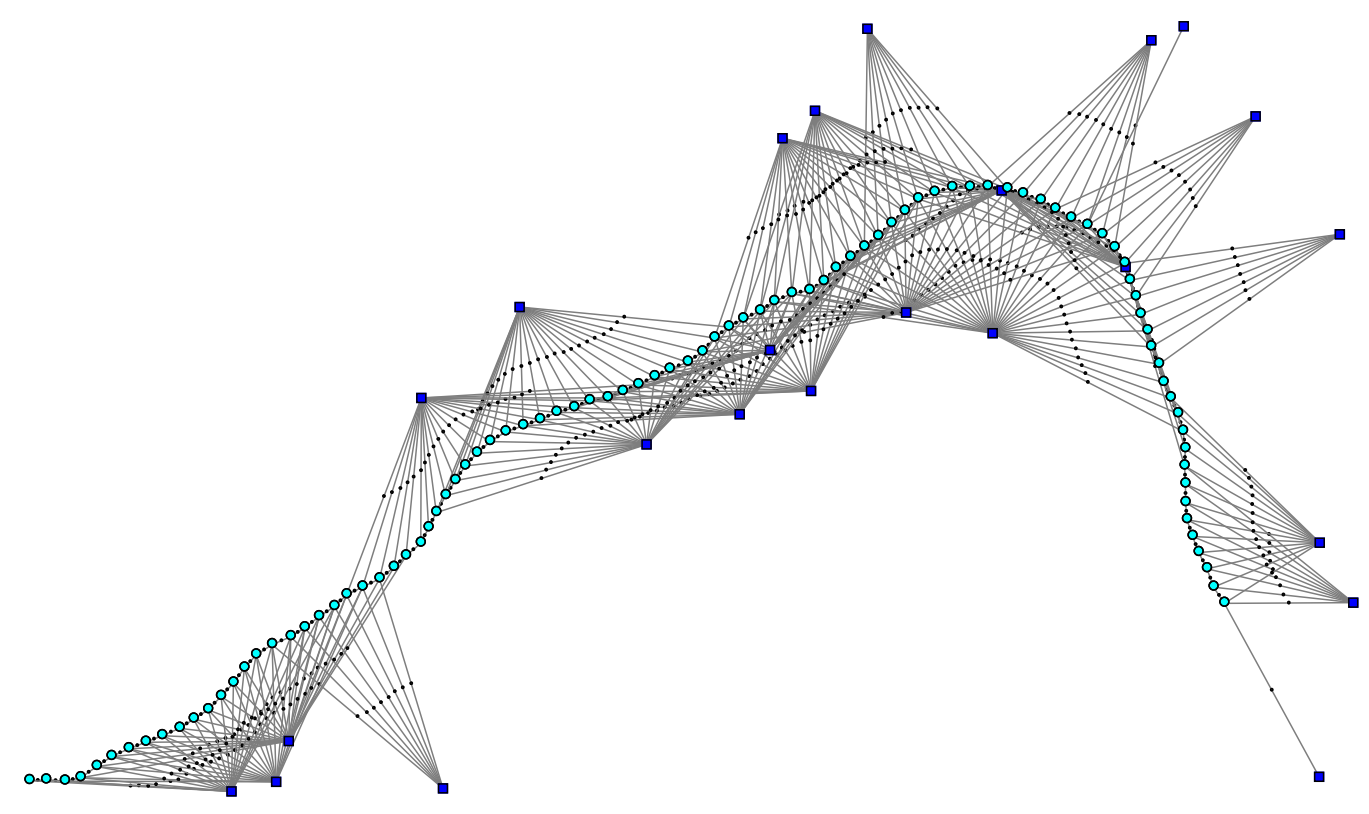
\includegraphics[width=0.9\linewidth]{Pictures/System_Modeling/Factor_Graphs/Example.png}
    \caption{Example of a factor graph in a simulated SLAM problem. Light blue circles represent the estimated robot trajectory, and dark blue squares represent observed landmarks. The connecting black edges/lines are factors, each defining a local probabilistic constraint between variables.\textsuperscript{\cite{factor_graphs}}}
    \label{fig:system-modeling-factor-graph-example}
\end{figure}

\newpage

\subsubsection{Mathematical Formulation}
A factor graph expresses the joint probability distribution of all system states as a product of smaller, locally defined functions. This can be written as:
$$
    p(\mathbf{x}) = \frac{1}{Z} \prod_{i=1}^{M} \phi_i(\mathbf{x}_i)
$$
where each factor $\phi_i(\mathbf{x}_i)$ represents a local probabilistic constraint involving only a subset of variables $\mathbf{x}_i$, and $Z$ is a normalization constant.  
\\ \\
In system modelling, these factors describe relationships such as motion models $f(\mathbf{x}, \mathbf{u})$ that connect consecutive states (See Equation \ref{eq:kinematics-motion-model}), measurement models $h(\mathbf{x})$ linking states to sensor observations (For example processed Side Scan Sonar 2D image), and prior terms that encode initial conditions. This factorization captures the conditional independence structure of the system and enables efficient and modular computation within probabilistic estimation frameworks.



\subsubsection{Integration in the System Model}
In this project, factor graphs are used to represent the complete state estimation problem by combining the INS motion model with processed measurements from the Side Scan Sonar within a unified probabilistic framework. The motion model defines the dynamic constraints between time steps, while the sonar derived landmark observations add measurement factors that update and refine the estimated trajectory within the overall system model.
 \clearpage
 \clearpage
\section{State Estimation}

intro to it
Bayes filter
KF + Talk about propagation Newton and also RK4 method :)
EKF
ESKF
UKF (WIth bias and all :D f() IMU model for that, + since quarternion, have to normalize after update the quarternion angle yesyes) + Alternative Sigma Point generation for better aproximation and stability
Some other that might be uselful for later just to mention, like ESKF or UKF for system Idtentification for hydrostatic and parameters and better model aproximation.
TUNING (NIS and other stuff to keep in mind)
State Variables at the end ie the ESKF variables that wahta we end up with


EKF vs ESKF (1 kind of state vs 2 kinds of states)
IMPORTANT: ESKF Covariance is of error state NOT nominal state!!!!!
explain why error state better than EKF


ESKF:
A and G are just aprocimations of DISCRETIZATION, but you can get a better dicreteziced system using kayley hamilton for these error matrix system. however more run time witch might not be good, so thats why usually we use the A and G defined already lol


 \clearpage
\section{Preintegration}
\subsection{Introduction}
In graph based SLAM, the preintegration method addresses the computational inefficiency caused by high frequency inertial measurements relative to low frequency exteroceptive sensors such as sonar. In a typical Side Scan Sonar SLAM (SSS SLAM) setup, a new sonar 2D map image is produced every few seconds at a rate of less thank 0.1 Hz, while the onboard IMU operates at several hundred hertz. If all IMU measurements were to be directly added to the factor graph as individual odometry factors by just simply using ESKF or UKF-M estimate, this would result in hundreds of redundant nodes between consecutive 2D sonar map frames. Such dense factor creation would significantly increase the computational load during optimization, while contributing limited additional information to the overall estimation process.
\\ \\
Preintegration resolves this problem by summarizing all IMU measurements between two 2D sonar map frames into a single compound odometry factor. This preintegrated factor represents the total relative motion, orientation change, and accumulated uncertainty over the integration interval, without introducing intermediate IMU states into the graph. The resulting factor provides the same essential motion constraints as full IMU integration using ESKF or UKF-M as Dead Reckoning estimate, but in a compact and computationally efficient form. This approach is particularly beneficial for SSS SLAM, where the sensor rate mismatch between the IMU and sonar is substantial.
\\ \\
The preintegration method uses the same INS motion model $f(x,u)$ as presented in Equation \ref{eq:kinematics-motion-model}, with minor modifications in how biases are handled and how the state propagation is performed. In contrast to the discrete propagation used in the State Estimation chapter described in Equation \ref{eq:state-estimation-discrete-propagartion}, preintegration assumes the accelerometer and gyroscope biases remain constant over the short integration window. This assumption simplifies the computation while retaining sufficient accuracy for most robotic applications.
\\ \\
The outcome of preintegration is a single, bias correctable odometry factor connecting two consecutive keyframes at the sonar update rate. This allows the SLAM system to maintain precise and consistent motion constraints while keeping the factor graph sparse. The approach achieves comparable accuracy to full state propagation methods such as ESKF or UKF-M but avoids the overhead associated with large numbers of intermediate factors.
\\ \\
Preintegration has been widely adopted in modern SLAM frameworks, including the Georgia Tech Smoothing and Mapping library (GTSAM), which provides dedicated classes for implementing preintegrated IMU factors discussed in later chapters of the thesis. The method was originally introduced for visual inertial odometry paper \cite{preintegration_camera_paper} and has been used in many modern SLAM problems such as for LiDAR and radar inertial fusion \cite{preintegration_radar_paper}. The same principles directly apply to sonar inertial systems, where the slow image acquisition rate makes preintegration a critical component for efficient factor graph optimization.
\begin{figure}[H]
    \centering
    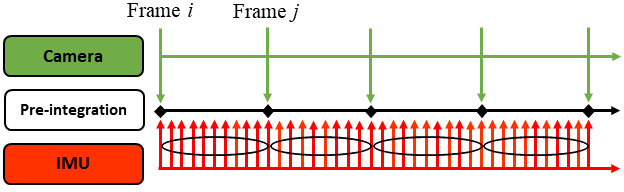
\includegraphics[width=1.0\linewidth]{Pictures/Preintegration/Introduction/Camera_IMU_example.jpg}
    \caption{Illustration of the sampling rate mismatch between an IMU and an exteroceptive sensor such as a camera or sonar. The IMU operates at hundreds of hertz, producing dense inertial measurements, while the sonar or camera generates new observations at a much lower rate. Preintegration combines all intermediate IMU readings into a single relative motion constraint that aligns with the moment a camera or sonar image is acquired.\textsuperscript{\cite{preintegration_camera_imu_picture}}}
    \label{fig:preintegration-camera-imu-example}
\end{figure}


 \clearpage
\subsection{Preintegration on Manifolds}
\subsubsection{INS Propagation Between IMU Samples}
The preintegration algorithm builds directly on the deterministic continuous time INS motion model defined in Equation \ref{eq:kinematics-motion-model}, where the system state is given by $\mathbf{x} = [\mathbf{p}_{b/O}^{n}, \mathbf{v}_{b/O}^{n}, \mathbf{q}, \mathbf{a}_b, \boldsymbol{\omega}_b]^\top$ and the input vector by $\mathbf{u} = [\mathbf{a}_m, \boldsymbol{\omega}_m]^\top$, as presented in Equation \ref{eq:kinematics-motion-model-states}. The same state representation is used here, consisting of position $\mathbf{p}$, velocity $\mathbf{v}$, and attitude $R(\mathbf{q})$, along with the accelerometer and gyroscope bias states $\mathbf{a}_b$ and $\boldsymbol{\omega}_b$. The motion model follows the same nominal kinematic equations as defined in the system modeling chapter, where the rigid body dynamics evolve according to the IMU measurements $(\mathbf{a}_m, \boldsymbol{\omega}_m)$ corrected by their respective biases. Hence, the same continuous time INS equations described in Equation \ref{eq:kinematics-motion-model} and the corresponding discrete form in Equation \ref{eq:state-estimation-discrete-propagartion} apply here.
\\ \\
In contrast to the full state estimator formulation used previously, which employed a 1st order Gauss Markov process for modeling bias drift, preintegration adopts a simpler Brownian motion bias model. This simplification is made because the preintegration window is short, and any bias evolution within this interval is small compared to the measurement noise and will be corrected later by the backend optimizer. The Brownian model is defined as
\begin{equation}
    \begin{aligned}
        \dot{\mathbf{a}}_b = \boldsymbol{\eta}_{a_b} \qquad \boldsymbol{\eta}_{a_b} \sim \mathcal{N}(0, \sigma_{a_b}^2 I_3) \\
        \dot{\boldsymbol{\omega}}_b = \boldsymbol{\eta}_{\omega_b} \qquad \boldsymbol{\eta}_{\omega_b} \sim \mathcal{N}(0, \sigma_{\omega_b}^2 I_3)
    \end{aligned}
    \label{eq:preintegration-bias-brownian-model}
\end{equation}
where $\boldsymbol{\eta}_{a_b}$ and $\boldsymbol{\eta}_{\omega_b}$ are zero mean Gaussian noise processes representing the bias random walk. The discrete time equivalent form becomes
\begin{equation}
    \begin{aligned}
        \mathbf{a}_{b,k+1} &= \mathbf{a}_{b,k} + \boldsymbol{\eta}_{a_b,d} \\
        \boldsymbol{\omega}_{b,k+1} &= \boldsymbol{\omega}_{b,k} + \boldsymbol{\eta}_{\omega_b,d}
    \end{aligned}
    \label{eq:preintegration-bias-propagartion}
\end{equation}
with $\operatorname{Cov}(\boldsymbol{\eta}_{a_b,d}) = \sigma_{a_b}^2 \Delta t I_3$ and $\operatorname{Cov}(\boldsymbol{\eta}_{\omega_b,d}) = \sigma_{\omega_b}^2 \Delta t I_3$. Over short preintegration intervals, these biases are assumed constant, meaning their change between IMU samples is negligible. The integration therefore proceeds using frozen bias estimates $\mathbf{a}_b$ and $\boldsymbol{\omega}_b$ from the start of the interval.
\\ \\
The nominal discrete time propagation of position, velocity, and rotation between IMU samples follows the same structure as the state estimation chapter in Equation \ref{eq:state-estimation-discrete-propagartion}, but is here expressed explicitly for clarity as
$$
    \begin{aligned}
        R_{k+1} &= R_k \exp([\boldsymbol{\omega}_{m,k} - \boldsymbol{\omega}_{b,k}]_\times \Delta t) \\
        v_{k+1} &= v_k + R_k(\mathbf{a}_{m,k} - \mathbf{a}_{b,k})\Delta t + \mathbf{g}\Delta t \\
        p_{k+1} &= p_k + v_k\Delta t + \tfrac{1}{2}R_k(\mathbf{a}_{m,k} - \mathbf{a}_{b,k})\Delta t^2 + \tfrac{1}{2}\mathbf{g}\Delta t^2
    \end{aligned}
$$
In this formulation, the index $k$ denotes consecutive IMU samples integrated at a high rate (typically hundreds of hertz). These samples are accumulated over the time interval between two keyframes $i$ and $j$, where each keyframe corresponds to a slower exteroceptive measurement such as a sonar 2D image frame. The goal of preintegration is to compress all intermediate IMU updates $(k=i, \ldots, j-1)$ into a single compound relative motion estimate connecting the two keyframes $i$ and $j$. 
\\ \\
The raw IMU outputs $\mathbf{a}_{m,k}$ and $\boldsymbol{\omega}_{m,k}$ represent the measured specific force and angular velocity in the body frame. The bias terms $\mathbf{a}_{b,k}$ and $\boldsymbol{\omega}_{b,k}$ are the current estimates of the accelerometer and gyroscope biases and are subtracted once within the propagation equations to obtain the corrected physical quantities. The resulting propagation is therefore already bias compensated and forms the deterministic foundation for the preintegration and subsequent error propagation steps described in the following sections.
\\ \\
At the beginning of each new preintegration interval $(t_j, t_{j+1}]$, the initial state $(R_i, v_i, p_i)$ is set equal to the optimized estimates from the previous keyframe, ie:
$$
    R_i = R_j^{\text{opt}}, \quad v_i = v_j^{\text{opt}}, \quad p_i = p_j^{\text{opt}}, \quad B_i = B_j^{\text{opt}}
$$
This ensures that the preintegration always starts from the most accurate state and bias estimates provided by the backend optimizer, maintaining temporal consistency across all keyframe intervals.



\subsubsection{Preintegration Initialization}
Preintegration is initialized at the time of keyframe $i$, corresponding to the most recent exteroceptive measurement such as a sonar frame. All IMU samples collected between keyframes $i$ and $j$ are subsequently integrated in the local coordinate frame of keyframe $i$. This ensures that the resulting preintegrated quantities describe motion relative to keyframe $i$ rather than the global frame, maintaining numerical stability and simplifying later optimization.
\\ \\
At the start of preintegration, the relative motion increments are initialized as
$$
    \Delta R_{ii} = I_3, \qquad
    \Delta v_{ii} = \mathbf{0}_3, \qquad
    \Delta p_{ii} = \mathbf{0}_3
$$
which represent, respectively, the initial relative rotation, velocity, and position between the same keyframe. These quantities form the starting point for integrating subsequent IMU samples.
\\ \\
The IMU bias used during preintegration is frozen at its current estimate from keyframe $i$, denoted by
$$
    B_i^{\text{preint}} = [\mathbf{a}_{b,i},\, \mathbf{\omega}_{b,i}]
$$
and is held constant throughout the preintegration interval $(t_i, t_j]$. The assumption of frozen bias is reasonable since the bias drift is slow compared to the short duration between keyframes, and any accumulated error is later corrected by the backend optimizer.
\\ \\
For uncertainty propagation, the Jacobians of the preintegrated quantities with respect to bias are initialized as
$$
    J_R^{\boldsymbol{\omega}_b} = J_v^{\mathbf{a}_b} = J_v^{\boldsymbol{\omega}_b} = J_p^{\mathbf{a}_b} = J_p^{\boldsymbol{\omega}_b} = 0
$$
These matrices are propagated forward with each IMU sample to capture how small bias perturbations affect the resulting preintegrated deltas, allowing efficient bias correction without re-integrating all IMU data.
\\ \\
All IMU readings are integrated relative to the orientation $R_i$ of the starting keyframe, ensuring that the computed preintegrated deltas $(\Delta R_{ij}, \Delta v_{ij}, \Delta p_{ij})$ remain expressed consistently in the local frame of keyframe $i$. The index $k$ denotes consecutive IMU samples integrated at a high rate (typically hundreds of hertz), while the index $j$ represents the current end of the ongoing preintegration interval. As new IMU data arrive, $j$ moves forward in time, meaning that $(\Delta R_{ij}, \Delta v_{ij}, \Delta p_{ij})$ are continuously updated until the next exteroceptive keyframe (eks sonar frame) is reached. Once keyframe $j$ is established, the accumulated deltas at that moment represent the complete preintegrated motion between frames $i$ and $j$.
\\ \\
This initialization therefore defines the starting state, bias configuration, and Jacobian setup for the recursive preintegration algorithm described in the following section.



\subsubsection{Preintegration Algorithm (Recursive Update)}
Once initialized, the preintegration proceeds recursively by integrating each incoming IMU measurement between the current keyframe $i$ and the evolving endpoint $j$. The integration runs at IMU rate (typically hundreds of hertz), using the frozen bias estimate $B_i^{\text{preint}} = [\mathbf{a}_{b,i}, \boldsymbol{\omega}_{b,i}]$. The preintegrated quantities $\Delta R_{ij}$, $\Delta v_{ij}$, and $\Delta p_{ij}$ are updated incrementally with every IMU sample $k$ according to
\begin{equation}
    \begin{aligned}
        \Delta R_{i,k+1} &= \Delta R_{i,k} \exp([\boldsymbol{\omega}_{m,k} - \boldsymbol{\omega}_{b,i}]_\times \Delta t) \\
        \Delta v_{i,k+1} &= \Delta v_{i,k} + \Delta R_{i,k}(\mathbf{a}_{m,k} - \mathbf{a}_{b,i})\Delta t \\
        \Delta p_{i,k+1} &= \Delta p_{i,k} + \Delta v_{i,k}\Delta t + \tfrac{1}{2}\Delta R_{i,k}(\mathbf{a}_{m,k} - \mathbf{a}_{b,i})\Delta t^2
    \end{aligned}
    \label{eq:preintegration-nominal-update}
\end{equation}
The exponential map $\exp([\cdot]_\times)$ ensures that the orientation update remains consistent on the manifold $SO(3)$, maintaining a valid rotation representation after each integration step. These updates are applied sequentially for all IMU samples within the preintegration window $(t_i, t_j]$.
\\ \\
The integration is performed in the local frame of keyframe $i$, meaning that all quantities $(\Delta R_{ij}, \Delta v_{ij}, \Delta p_{ij})$ are expressed relative to the orientation $R_i$. The index $k$ refers to the current IMU sample, while $j$ marks the progressively advancing endpoint of the preintegration interval as new IMU data arrive. When the next exteroceptive keyframe $j$ (eks a 2D sonar image) is received, the accumulated deltas represent the complete preintegrated motion between the two complete keyframes $i$ and $j$.
\\ \\
This recursive integration scheme effectively compresses all high frequency IMU updates into a single relative motion constraint while preserving the nonlinear structure of the underlying kinematics on $SE(3)$. It forms the foundation for the subsequent Jacobian propagation and covariance update described in the following sections.



\subsubsection{Bias Jacobian Propagation}
The bias Jacobian propagation captures how small changes in accelerometer and gyroscope biases affect the preintegrated quantities $(\Delta R_{ij}, \Delta v_{ij}, \Delta p_{ij})$. Although the biases are assumed constant within each preintegration interval, they are later refined by the optimizer. By maintaining their partial derivatives, the preintegration can be corrected efficiently without re-integrating all IMU data. The Jacobians represent the first-order sensitivity of the preintegrated deltas with respect to the bias states:
$$
    J_R^{\boldsymbol{\omega}_b} = \frac{\partial\,\text{Log}(\Delta R_{ij})}{\partial \boldsymbol{\omega}_b}, \quad
    J_v^{\mathbf{a}_b} = \frac{\partial\,\Delta v_{ij}}{\partial \mathbf{a}_b}, \quad
    J_v^{\boldsymbol{\omega}_b} = \frac{\partial\,\Delta v_{ij}}{\partial \boldsymbol{\omega}_b}, \quad
    J_p^{\mathbf{a}_b} = \frac{\partial\,\Delta p_{ij}}{\partial \mathbf{a}_b}, \quad
    J_p^{\boldsymbol{\omega}_b} = \frac{\partial\,\Delta p_{ij}}{\partial \boldsymbol{\omega}_b}
$$
The $\text{Log}(\cdot)$ operator in $J_R^{\boldsymbol{\omega}_b}$ maps the incremental rotation $\Delta R_{ij}$ from the manifold $SO(3)$ to its tangent space $\mathfrak{so}(3)$, allowing the small rotation errors to be represented as 3D vectors in Euclidean space where derivatives can be taken linearly (See Equations \ref{eq:lie-groups-and-manifold-exponential} and \ref{eq:lie-groups-and-manifold-logarithmic}). All Jacobians are initialized to zero at the start of preintegration and propagated at every IMU timestep using 1st order linearization:
$$
    J(t+\Delta t) = J(t) + \frac{\partial(\Delta R, \Delta v, \Delta p)}{\partial b}\Delta t
$$
No higher order bias dynamics are modeled since bias drift is slow and follows a Brownian process. Given the nominal preintegration updates with Equation \ref{eq:preintegration-nominal-update} the bias Jacobians evolve as
$$
    \begin{aligned}
    J_R^{\boldsymbol{\omega}_b}(k+1) &\approx J_R^{\boldsymbol{\omega}_b}(k) - \Delta R_{i,k}\Gamma_1\Delta t \\
    J_v^{\mathbf{a}_b}(k+1) &\approx J_v^{\mathbf{a}_b}(k) - \Delta R_{i,k}\Delta t \\
    J_v^{\boldsymbol{\omega}_b}(k+1) &\approx J_v^{\boldsymbol{\omega}_b}(k) - \Delta R_{i,k}[\mathbf{a}_{m,k} - \mathbf{a}_{b,i}]_\times J_R^{\boldsymbol{\omega}_b}(k)\Delta t \\
    J_p^{\mathbf{a}_b}(k+1) &\approx J_p^{\mathbf{a}_b}(k) + J_v^{\mathbf{a}_b}(k)\Delta t - \tfrac{1}{2}\Delta R_{i,k}\Delta t^2 \\
    J_p^{\boldsymbol{\omega}_b}(k+1) &\approx J_p^{\boldsymbol{\omega}_b}(k) + J_v^{\boldsymbol{\omega}_b}(k)\Delta t - \tfrac{1}{2}\Delta R_{i,k}[\mathbf{a}_{m,k} - \mathbf{a}_{b,i}]_\times J_R^{\boldsymbol{\omega}_b}(k)\Delta t^2
    \end{aligned}
$$
where $\Gamma_1$ is the 1st order right Jacobian of $SO(3)$, evaluated at the small rotation vector $\boldsymbol{\phi}_k = (\boldsymbol{\omega}_{m,k} - \boldsymbol{\omega}_{b,i})\Delta t$. It maps perturbations in the Lie algebra (tangent space) to perturbations on the manifold, ensuring correct rotation updates for small angular increments (See Equations \ref{eq:lie-groups-and-manifold-exponential} and \ref{eq:lie-groups-and-manifold-logarithmic}). In closed form
$$
    \Gamma_1(\boldsymbol{\phi}_k) = I_3 - \frac{1 - \cos\|\boldsymbol{\phi}_k\|}{\|\boldsymbol{\phi}_k\|^2}[\boldsymbol{\phi}_k]_\times + \frac{\|\boldsymbol{\phi}_k\| - \sin\|\boldsymbol{\phi}_k\|}{\|\boldsymbol{\phi}_k\|^3}[\boldsymbol{\phi}_k]_\times^2
$$
and for small rotations, it can be approximated as
$$
    \Gamma_1(\boldsymbol{\phi}_k) \approx I_3 - \tfrac{1}{2}[\boldsymbol{\phi}_k]_\times
$$
This Jacobian maintains manifold consistency by correctly relating incremental angular changes to their corresponding local linearizations on $SO(3)$. The $\text{Log}(\cdot)$ operator in $J_R^{\boldsymbol{\omega}_b}$ projects the rotational error from the manifold $SO(3)$ to the tangent space $\mathfrak{so}(3)$, providing a linear representation of small rotation errors that enables differentiation with respect to the gyroscope bias.
\\ \\
Finally, the Jacobians computed at each IMU timestep are accumulated over the full preintegration interval $(t_i, t_j]$ to form the total bias sensitivity between keyframes $i$ and $j$. This accumulation corresponds to summing the incremental contributions from each IMU update:
$$
    J_R^{\boldsymbol{\omega}_b} = \sum_{k=i}^{j-1} J_R^{\boldsymbol{\omega}_b}(k), \qquad
    J_v^{\mathbf{a}_b} = \sum_{k=i}^{j-1} J_v^{\mathbf{a}_b}(k), \qquad
    J_v^{\boldsymbol{\omega}_b} = \sum_{k=i}^{j-1} J_v^{\boldsymbol{\omega}_b}(k), \qquad
    J_p^{\mathbf{a}_b} = \sum_{k=i}^{j-1} J_p^{\mathbf{a}_b}(k), \qquad
    J_p^{\boldsymbol{\omega}_b} = \sum_{k=i}^{j-1} J_p^{\boldsymbol{\omega}_b}(k)
$$
Thus, each Jacobian term represents the cumulative 1st order effect of bias perturbations over all IMU samples between the two keyframes. These accumulated Jacobians form the final bias correction matrices used in the subsequent preintegration update step.



\subsubsection{Bias Re-Linearization Using Accumulated Jacobians}
When the optimizer send update and corrects the bias estimates, the stored preintegrated quantities must be re-linearized to stay consistent with the new bias values. Instead of re-integrating all IMU samples, this correction is efficiently performed using the accumulated Jacobians computed during preintegration.
\\ \\
The bias correction increment is defined as
$$
    \delta B_i = [\delta \mathbf{a}_b, \, \delta \boldsymbol{\omega}_b] = B_i^{\text{opt}} - B_i^{\text{preint}}
$$
where $B_i^{\text{preint}}$ is the frozen bias used during preintegration and $B_i^{\text{opt}}$ is the updated bias from the optimizer. The corrected preintegrated quantities are obtained by applying a 1st order correction using the propagated Jacobians:
$$
    \begin{aligned}
        \Delta R_{ij}^{*} &\approx \Delta R_{ij}\exp(J_R^{\boldsymbol{\omega}_b}\delta\boldsymbol{\omega}_b) \\
        \Delta v_{ij}^{*} &\approx \Delta v_{ij} + J_v^{\mathbf{a}_b}\delta\mathbf{a}_b + J_v^{\boldsymbol{\omega}_b}\delta\boldsymbol{\omega}_b \\
        \Delta p_{ij}^{*} &\approx \Delta p_{ij} + J_p^{\mathbf{a}_b}\delta\mathbf{a}_b + J_p^{\boldsymbol{\omega}_b}\delta\boldsymbol{\omega}_b
    \end{aligned}
$$
where $(\cdot)^*$ denotes the bias corrected preintegrated quantities. The $\exp(\cdot)$ operator maps the small correction $J_R^{\boldsymbol{\omega}_b}\delta\boldsymbol{\omega}_b$ from the tangent space back onto the rotation manifold $SO(3)$, ensuring consistent attitude updates (See Equations \ref{eq:lie-groups-and-manifold-exponential} and \ref{eq:lie-groups-and-manifold-logarithmic}).
\\ \\
The accumulated Jacobians $(J_R^{\boldsymbol{\omega}_b}, J_v^{\mathbf{a}_b}, J_v^{\boldsymbol{\omega}_b}, J_p^{\mathbf{a}_b}, J_p^{\boldsymbol{\omega}_b})$ compactly represent the total 1st order sensitivity of the preintegrated deltas to bias changes across the entire preintegration interval $(t_i, t_j]$. Using these, the optimizer can instantly re-evaluate the preintegrated measurements without reprocessing any IMU data, maintaining full geometric consistency while minimizing computational cost.



\subsubsection{Predicted Motion Reconstruction}
Once the preintegrated measurements have been bias corrected, they can be used to reconstruct the nominal motion between the two keyframes $i$ and $j$. This reconstruction provides the predicted navigation state $(\hat{R}_j, \hat{v}_j, \hat{p}_j)$ at keyframe $j$, given the known state $(R_i, v_i, p_i)$ at keyframe $i$ and the corrected preintegrated deltas $(\Delta R_{ij}^{*}, \Delta v_{ij}^{*}, \Delta p_{ij}^{*})$.
\\ \\
The nominal motion prediction is obtained as
$$
    \begin{aligned}
        \hat{R}_j &= R_i \Delta R_{ij}^{*} \\
        \hat{v}_j &= v_i + \mathbf{g}\Delta t_{ij} + R_i \Delta v_{ij}^{*} \\
        \hat{p}_j &= p_i + v_i\Delta t_{ij} + \tfrac{1}{2}\mathbf{g}\Delta t_{ij}^2 + R_i \Delta p_{ij}^{*}
    \end{aligned}
$$
where $\mathbf{g}$ is the gravity vector expressed in the navigation frame, and $\Delta t_{ij}$ is the total elapsed time between keyframes $i$ and $j$. The predicted quantities $(\hat{R}_j, \hat{v}_j, \hat{p}_j)$ represent the best estimate of the motion over the interval $(t_i, t_j]$ using only IMU data.
\\ \\
The resulting predicted state for keyframe $j$ is compactly expressed as
$$
    \hat{X}_j =
    \begin{bmatrix}
        \hat{p}_j \\
        \hat{v}_j \\
        \hat{R}_j
    \end{bmatrix}
$$
which serves as the nominal prior for the next optimization step and ensures temporal consistency across keyframes.



\subsubsection{Predicted Bias Reconstruction}
In addition to predicting the nominal motion, the IMU bias state must also be propagated between keyframes. The bias follows the Brownian random walk model introduced earlier in Equation \ref{eq:preintegration-bias-brownian-model}, which assumes slow, uncorrelated drift over short time intervals.  
\\ \\
The discrete time bias propagation between consecutive IMU samples is given by Equation \ref{eq:preintegration-bias-propagartion}, where the bias mean remains constant, but its uncertainty grows due to the additive white noise processes $\boldsymbol{\eta}_{a_b,d}$ and $\boldsymbol{\eta}_{\omega_b,d}$. Over the preintegration interval $(t_i, t_j]$, this simplifies to
$$
    \begin{aligned}
        \hat{\mathbf{a}}_{b,j} &= \mathbf{a}_{b,i} \\
        \hat{\boldsymbol{\omega}}_{b,j} &= \boldsymbol{\omega}_{b,i}
    \end{aligned}
$$
indicating that the bias mean is held constant throughout the preintegration. The corresponding uncertainty growth due to the Brownian process is captured later through the bias covariance matrix $Q_b$.  
\\ \\
The predicted bias state at keyframe $j$ is therefore
$$
    \hat{B}_j = 
    \begin{bmatrix}
        \hat{\mathbf{a}}_{b,j} \\
        \hat{\boldsymbol{\omega}}_{b,j}
    \end{bmatrix}
    =
    \begin{bmatrix}
        \mathbf{a}_{b,i} \\
        \boldsymbol{\omega}_{b,i}
    \end{bmatrix}
$$
and is passed together with the predicted motion state $\hat{X}_j$ to the backend optimizer for joint correction and relinearization.



\subsubsection{Preintegration Covariance Propagation}
In addition to the predicted navigation states, the associated uncertainty must also be propagated to quantify the confidence of the preintegrated motion estimate. This covariance describes how IMU process noise accumulates over the preintegration interval and directly influences the weighting of the IMU constraint during optimization.  
\\ \\
The propagation of covariance during IMU preintegration follows the same mathematical principles as the ESKF formulation presented in the State Estimation chapter. In particular, it corresponds to a reduced version of the full error state INS model in Equation \ref{eq:state-estimation-error-state-dynamics}, using only the first three state components, position, velocity, and attitude. The bias states are omitted here since their uncertainty is treated separately under the Brownian motion bias model described previously. The resulting reduced error state vector is therefore defined as
$$
    \delta \mathbf{x} =
    \begin{bmatrix}
        \delta \mathbf{p} \\
        \delta \mathbf{v} \\
        \delta \mathbf{q}
    \end{bmatrix}
$$
where $\delta\mathbf{q}$ represents the small quaternion attitude error, approximated as in Equation \ref{eq:state-estimation-error-states} using the small angle representation
$$
    \delta\mathbf{q} \approx
    \begin{bmatrix}
        1 \\
        \tfrac{1}{2}\delta\boldsymbol{\theta}
    \end{bmatrix}
$$
This small angle approximation allows attitude uncertainty to be represented in a minimal 3D tangent space, preserving the quaternion manifold structure while maintaining linear error propagation.
\paragraph{Continuous Time Error Dynamics} \mbox{}\\[0.5em] \noindent
The continuous time linearized error dynamics for the preintegration process directly mirror the first three block rows of the ESKF system matrix $A(\mathbf{x})$ in Equation \ref{eq:state-estimation-error-state-linear-time-varying-matrices}. Neglecting the bias terms yields:
$$
    \delta \dot{\mathbf{x}}(t) = A(t)\delta \mathbf{x}(t) + B(t)\mathbf{n}(t)
$$
with
$$
    A(t) =
    \begin{bmatrix}
        0 & I_3 & 0 \\
        0 & 0 & -R_i^\top R(t)[\mathbf{a}_m(t) - \mathbf{a}_b]_\times \\
        0 & 0 & -[\boldsymbol{\omega}_m(t) - \boldsymbol{\omega}_b]_\times
    \end{bmatrix},
    \qquad
    B(t) =
    \begin{bmatrix}
        0 & 0 \\
        -R_i^\top R(t) & 0 \\
        0 & -I_3
    \end{bmatrix}
$$
Here $R_i^\top R(t)$ represents the relative rotation between the start keyframe $i$ and the current IMU orientation $R(t)$, ensuring that all quantities remain expressed in the local frame of keyframe $i$. The noise term $\mathbf{n}(t) = [\mathbf{n}_a, \mathbf{n}_\omega]^\top$ corresponds to the same white Gaussian IMU noise components used in the ESKF process model.
\paragraph{Discretization and Covariance Propagation} \mbox{}\\[0.5em] \noindent
As discussed in in previous chapters under State Estimation in ESKF discretization section (See Equation \ref{eq:state-estimation-error-state-dynamics-discretized}), discretization of the continuous error dynamics is necessary for digital implementation. Similar to the ESKF, the Zero Order Hold (ZOH) method can be applied here, or similar methods, assuming the IMU inputs and noise remain constant within each sampling interval $\Delta t$. The discrete time covariance propagation is therefore given by
$$
    P_{IMU,k+1} = A_k P_{IMU,k} A_k^\top + B_k Q_\eta B_k^\top
$$
where
$$
    Q_\eta = \operatorname{diag}(\sigma_a^2 I_3, \sigma_\omega^2 I_3)
$$
is the continuous time IMU noise covariance, scaled by the timestep $\Delta t$ within the discretization. This formulation is mathematically equivalent to the discretized process noise computation in Equation \ref{eq:state-estimation-error-state-dynamics-discretized}, except that only the preintegrated motion subspace $(\mathbf{p}, \mathbf{v}, \mathbf{q})$ is considered. The initial covariance at the start of preintegration is set to
$$
    P_{IMU,ii} = 0_{9\times9},
$$
indicating no accumulated uncertainty at keyframe $i$. As IMU samples are integrated, $P_{IMU,k}$ evolves recursively with each step, incorporating both linearized system dynamics and sensor noise effects.
\paragraph{Resulting Preintegration Covariance} \mbox{}\\[0.5em] \noindent
After integrating all IMU measurements between keyframes $i$ and $j$, the final propagated covariance is obtained as
$$
    P_{IMU,ij} = P_{IMU,k_{\text{end}}}
$$
This $9\times9$ covariance matrix represents the total uncertainty of the preintegrated relative motion $(\Delta p_{ij}, \Delta v_{ij}, \Delta R_{ij})$ in the local frame of keyframe $i$. The inverse covariance, referred to as the information matrix,
$$
    \Lambda_{IMU,ij} = P_{IMU,ij}^{-1}
$$
is used to weight the IMU factor in the nonlinear optimizers such as iSAM2 discussed in later chapters. A higher $\Lambda_{IMU,ij}$ corresponds to greater trust in the IMU preintegration constraint, while a lower weight allows more correction from exteroceptive sensor updates such as sonar or vision.  
\\ \\
In summary, this preintegration covariance propagation step is mathematically identical to the error state covariance propagation in the ESKF (Equations \ref{eq:state-estimation-error-state-dynamics}-\ref{eq:state-estimation-error-state-dynamics-discretized}), except that it operates on the reduced state $(\mathbf{p}, \mathbf{v}, \mathbf{q})$ and uses the local frame of keyframe $i$. This reduction significantly improves computational efficiency while maintaining consistency with the underlying inertial error dynamics.



\subsubsection{Bias Covariance Propagation}
In parallel with the preintegrated motion covariance, the uncertainty of the IMU bias states must also be propagated between keyframes. As introduced in Equation \ref{eq:preintegration-bias-brownian-model}, both accelerometer and gyroscope biases follow a Brownian random walk process, representing slow stochastic drift with zero mean. Over the short duration of a preintegration interval, the bias means remain effectively constant, while their uncertainty increases linearly with time.  
\\ \\
Applying the same discretization method used for the preintegration covariance like ZOH or similar methods (see Equation \ref{eq:state-estimation-error-state-dynamics-discretized}), the discrete time bias covariance propagation is given by
$$
    P_{b,ij} =
    \begin{bmatrix}
        \sigma_{a_b}^2 I_3 & 0 \\
        0 & \sigma_{\omega_b}^2 I_3
    \end{bmatrix}
    \Delta t_{ij}
$$
This represents the accumulated uncertainty in the bias states between keyframes $i$ and $j$, arising from the continuous time noise processes $\boldsymbol{\eta}_{a_b}$ and $\boldsymbol{\eta}_{\omega_b}$. The bias covariance evolves independently from the preintegrated motion covariance since the bias random walk is assumed uncorrelated with the instantaneous IMU measurement noise.  
\\ \\
The corresponding bias information matrix is therefore defined as
$$
    \Lambda_{b,ij} = P_{b,ij}^{-1}
$$
and represents the statistical weighting of the bias factor in the optimizer. This ensures that the bias evolution constraint contributes independently from the motion factor, allowing consistent and decoupled correction of both motion and bias estimates during optimization.



\subsubsection{Algorithm Summary}
The complete preintegration procedure can be summarized as follows:
\begin{itemize}
    \item \textbf{Initialization:}  
    Set $\Delta R_{ii} = I_3$, $\Delta v_{ii} = 0$, $\Delta p_{ii} = 0$, and initialize bias Jacobians $J = 0$.  
    Freeze bias estimate $B_i^{\text{preint}} = [\mathbf{a}_{b,i}, \boldsymbol{\omega}_{b,i}]$

    \item \textbf{Recursive IMU Integration:}  
    Integrate all IMU samples $(\mathbf{a}_{m,k}, \boldsymbol{\omega}_{m,k})$ between keyframes $i$ and $j$ to obtain  
    $\Delta R_{ij}, \Delta v_{ij}, \Delta p_{ij}$

    \item \textbf{Bias Jacobian Propagation:}  
    Propagate and accumulate $J_R^{\boldsymbol{\omega}_b}$, $J_v^{\mathbf{a}_b}$, $J_v^{\boldsymbol{\omega}_b}$, $J_p^{\mathbf{a}_b}$, $J_p^{\boldsymbol{\omega}_b}$

    \item \textbf{Bias Correction:}  
    Apply bias correction using accumulated Jacobians to get  
    $\Delta R_{ij}^{*}, \Delta v_{ij}^{*}, \Delta p_{ij}^{*}$

    \item \textbf{Predicted State Reconstruction:}  
    Compute $\hat{R}_j, \hat{v}_j, \hat{p}_j$ from $(R_i, v_i, p_i)$ and $(\Delta R_{ij}^{*}, \Delta v_{ij}^{*}, \Delta p_{ij}^{*})$

    \item \textbf{Predicted Bias Reconstruction:}  
    Propagate $\hat{B}_j = [\hat{\mathbf{a}}_{b,j}, \hat{\boldsymbol{\omega}}_{b,j}] = [\mathbf{a}_{b,i}, \boldsymbol{\omega}_{b,i}]$

    \item \textbf{State Covariance Propagation:}  
    Compute $P_{IMU,ij}$ and corresponding information matrix $\Lambda_{IMU,ij} = P_{IMU,ij}^{-1}$

    \item \textbf{Bias Covariance Propagation:}  
    Compute $P_{b,ij}$ and corresponding information matrix $\Lambda_{b,ij} = P_{b,ij}^{-1}$

    \item \textbf{Output:}  
    Return $(\Delta R_{ij}^{*}, \Delta v_{ij}^{*}, \Delta p_{ij}^{*}, \hat{B}_j, P_{IMU,ij}, P_{b,ij}, \Lambda_{IMU,ij}, \Lambda_{b,ij})$
\end{itemize}
 \clearpage
\subsection{Factor Construction}
\subsubsection{Factor Graph Formulation}
The optimizer operates on a factor graph representation of the estimation problem, where each node corresponds to a keyframe state and each edge, or factor, represents a probabilistic constraint derived from sensor measurements. For the preintegration framework to function within this optimization structure, the outputs from the preintegration algorithm must be converted into factors that connect consecutive keyframes. These factors define how motion and bias estimates evolve between time steps and provide the necessary mathematical relationships that the optimizer uses to minimize overall error.  
\\ \\
The factor graph formulation is crucial because it transforms the continuous time IMU dynamics into discrete, optimization ready constraints. Each factor contributes a residual that measures the discrepancy between the predicted and observed relationships of connected keyframes. During optimization, all residuals are jointly minimized to produce the most consistent estimate of both motion and bias states over time.  
\\ \\
In the context of IMU preintegration, two distinct but related factors are constructed. The first one is the IMU preintegration factor, which captures the relative motion between keyframes using the preintegrated measurements. The second one is the bias evolution factor, which models the slow stochastic drift of accelerometer and gyroscope biases. Together, these form the complete inertial constraint within the factor graph, allowing the optimizer to refine all state and bias variables simultaneously and propagate the optimal corrected state back into the next preintegration cycle.  
\\ \\
Once the optimization converges, the updated states $(R_j^{\text{opt}}, v_j^{\text{opt}}, p_j^{\text{opt}})$ and biases $B_j^{\text{opt}}$ are extracted from the graph and used to initialize the next preintegration interval $(t_j, t_{j+1}]$ and then constructing the factors again. This recursive update maintains temporal consistency between keyframes and ensures that each new preintegration step starts from the best available estimate.



\subsubsection{IMU Preintegration Factor}
This factor represents the relative motion constraint between keyframes $i$ and $j$ based on all IMU data integrated over the interval $(t_i, t_j]$. It enforces consistency between the estimated states $(R_i, v_i, p_i)$ and $(R_j, v_j, p_j)$ and the preintegrated measurements $(\Delta R_{ij}^{*}, \Delta v_{ij}^{*}, \Delta p_{ij}^{*})$ computed previously.  
\\ \\
Here, $R_i$, $v_i$, and $p_i$ correspond to the optimized state estimates from the previous keyframe, denoted as $R_i^{\text{opt}}$, $v_i^{\text{opt}}$, and $p_i^{\text{opt}}$, provided by the backend optimizer. Similarly, $R_j$, $v_j$, and $p_j$ represent the current state estimates under optimization, denoted as $\hat{R}_j$, $\hat{v}_j$, and $\hat{p}_j$. The preintegrated quantities $(\Delta R_{ij}^{*}, \Delta v_{ij}^{*}, \Delta p_{ij}^{*})$ are fixed measurements obtained from the preintegration process and serve as the relative motion observation linking these two states.
\\ \\
The residual formulation is given as
$$
    r_{\text{IMU}}^{ij} =
    \begin{bmatrix}
        \log((\Delta R_{ij}^{*})^\top R_i^\top R_j) \\
        R_i^\top (v_j - v_i - g\Delta t_{ij}) - \Delta v_{ij}^{*} \\
        R_i^\top (p_j - p_i - v_i \Delta t_{ij} - \tfrac{1}{2} g \Delta t_{ij}^2) - \Delta p_{ij}^{*}
    \end{bmatrix}
$$
Each residual term penalizes deviation from the preintegrated motion predicted by the IMU. The factor is weighted by the corresponding information matrix $\Lambda_{IMU,ij} = P_{IMU,ij}^{-1}$, defining its confidence based on accumulated IMU noise. 
\\ \\
This single factor efficiently summarizes hundreds of raw IMU readings, maintaining accuracy while drastically reducing computational cost.



\subsubsection{Bias Evolution Factor}
To maintain bias consistency between keyframes, a separate factor enforces smooth bias evolution according to the Brownian motion model.  
\\ \\
Here, $B_i$ represents the optimized bias estimate from the previous keyframe, denoted as $B_i^{\text{opt}} = [\mathbf{a}_{b,i}^{\text{opt}},\, \boldsymbol{\omega}_{b,i}^{\text{opt}}]^\top$, while $B_j$ corresponds to the current bias state being optimized, denoted as $\hat{B}_j = [\hat{\mathbf{a}}_{b,j},\, \hat{\boldsymbol{\omega}}_{b,j}]^\top$.  
\\ \\
The residual formulation is given as
$$
    r_{\text{b}}^{ij} = B_j - B_i
$$
weighted by the bias information matrix $\Lambda_{b,ij} = P_{b,ij}^{-1}$.  
\\ \\
This factor captures the slow, random drift of gyroscope and accelerometer biases over time and ensures stable long-term estimation.  

 \clearpage

 \clearpage
\section{Local Map Generation}

All use State estimates and measuremnt model h() here

Also when generating map locally we build it from sonar 1D images to a 2D recontruction, this takes time and this image is what is then processed and fed into SLAM
In adition next step we take with the last 1/3rd or the old image and generate a new image that is 2/3 new, this then becomes new 3/3 image that gets fed into SLAM and so forth
This is done so that data asocaition we dont cut off crucial info between frames and Data Sdociation and landmark detection can extract features again here.

Swath Processing

Cartesian Mapping

Feature Extraction (Landmark Detection) \clearpage
\section{Data Association}


Gating (Mahalanobis)

matching/tracking

Also talk about loop closures

produce measurement factors for optimizer \clearpage
\section{Optimizers}
\subsection{Introduction}
Introduce Optimizers \clearpage
\subsection{iSAM}
\subsubsection{Getting to SLAM update step}
Before computing a good estimate, defining simple models for robot motion and sensor observations is crucial. The motion model describes state evolution, and the measurement model describes sensor readings. States are $x_i$ for robot poses, controls are $u_i$, and measurements are $z_k$ for landmarks. Stack all unknowns into $\theta$, poses and landmarks.
\\ \\
Motion (process) model:
$$
    \begin{aligned}
        x_i = f_{i}(x_{i-1}, u_i) + w_i \\ 
        w_i \sim N(0, Q_i) \qquad
    \end{aligned}
$$
Given the previous state $x_{i-1}$ and control $u_i$, the next state $x_i$ comes from a model $f$ plus uncertainty noise in the model itself $w_i$. This uncertainty captures things like currents, slip, and actuator errors. $f_i$ can be a discrete time dynamics update or use plain odometry. Assuming Gaussian $w_i$ is a handy start so MAP becomes least squares. Later this uncertainty model can be switched to robust or heavy tailed noise model if needed.
\\ \\
Measurement model:
$$
    \begin{aligned}
        z_k = h_{k}(x_{i_k}, l_{j_k}) + v_k \\ 
        v_k \sim N(0, R_k) \qquad
    \end{aligned}
$$
Each measurement $z_k$ depends on state $x_{i_k}$ and landmarks $l_{j_k}$ transformed using measurement transform function $h_{k}(\cdot)$, this allows state estimate to become estimated measurement position. In addition this measurement has noise $v_k$ witch is modeled as Gaussian noise for simplifications later on when calculating.
\\ \\
Prior:
$$
    \begin{aligned}
        x_0 \sim N(\mu_{0}, \Sigma_{0})
    \end{aligned}
$$
A prior anchors the graph (otherwise the problem is underdetermined up to a global transform). It can encode GPS at the start, a known dock pose, or simply a weak ``zero'' prior to fix gauge.
\\ \\
Predictions should match measurements. In a perfect world, every residual (prediction minus measurement) would be zero. In practice, model errors and sensor noise make the residuals nonzero. Estimation is about choosing the state update that makes all residuals as small and as statistically consistent as possible.
\\ \\
This is where MAP algorithm comes in. MAP (Maximum A Posteriori) is the principled way to fuse everything we know. A prior on the state, the motion model, and all measurements. It combines them through probability, weighting each residual by its uncertainty. With Gaussian noise, the negative log posterior becomes a sum of squared (weighted) residuals. That gives us a single objective to minimize, where more reliable terms (small covariance) count more. This is better than ad hoc weighting and naturally handles many sensors.
\\ \\
Motion and measurement functions are nonlinear (angles, rotations, ranges). Minimizing the nonlinear MAP cost directly is hard. Linearization lets us solve it iteratively. At the current estimate approximate the nonlinear functions by their first order Taylor expansion, solve a linear least squares problem for a small increment, update the estimate, and repeat. This is all shown in the iSAM paper \cite{iSAM_paper} where linearized forms of the system becomes:
\begin{equation}
    \begin{aligned}
        f_{i}(x_{i-1}, u_i) - x_i \approx (F_{i}^{i-1}\Delta x_{i-1} - \Delta x_{i}) - a_i \\
        \left.F_{i}^{i-1} := \frac{\partial f_{i}(x_{i-1}, u_i)}{\partial x_{i-1}}\right|_{x_{i-1}^{0}} \\ 
        a_i = x_{i-1}^{0} - f_{i}(x_{i-1}^{0}, u_i)
    \end{aligned}
    \label{eq:optimizer-iSAM-linearized-odometry}
\end{equation}
\begin{equation}
    \begin{aligned}
        h_{k}(x_{i-1}, u_i) - z_k \approx (H_{k}^{i_k}\Delta x_{i_k} - J_{k}^{j_k} \Delta l_{j_k}) - c_k \\
        \left.H_{k}^{i_k} := \frac{\partial h_{k}(x_{i_k}, l_{j_k})}{\partial x_{i_k}}\right|_{(x_{i_k}^{0}, l_{j_k}^{0})} \\ 
        \left.J_{k}^{j_k} := \frac{\partial h_{k}(x_{i_k}, l_{j_k})}{\partial l_{j_k}}\right|_{(x_{i_k}^{0}, l_{j_k}^{0})} \\ 
        c_k = z_{k} - h_{k}(x_{i_k}^{0}, l_{j_k}^{0})
    \end{aligned}
    \label{eq:optimizer-iSAM-linearized-measurement}
\end{equation}
\\ \\
Plug the linearized odometry \eqref{eq:optimizer-iSAM-linearized-odometry} and measurement \eqref{eq:optimizer-iSAM-linearized-measurement} models into a single objective over the stacked increment vector $\Delta\theta$ (all pose and landmark updates). The goal is to pick the small change $\Delta\theta^{*}$ that jointly reduces all linearized residuals. Each factor becomes a linear row in the relevant increments. 
\\ \\
For an odometry factor $i$, the linearized residual is
$$
r_i^{\text{odo}}=F_i^{\,i-1}\Delta x_{i-1}+G_i^{\,i}\Delta x_i-a_i,
$$
where $F$ and $G$ are the odometry Jacobians. Because odometry constrains the relative change between $x_{i-1}$ and $x_i$, the block on $\Delta x_i$ is $-I$ ($G_i^{\,i}=-I$). Here $a_i$ is the current odometry prediction error.
\\ \\
For a measurement factor $k$ connecting pose $x_{i_k}$ to landmark $l_{j_k}$, the residual is
$$
r_k^{\text{meas}}=H_k^{\,i_k}\Delta x_{i_k}+J_k^{\,j_k}\Delta l_{j_k}-c_k,
$$
with $H$ and $J$ the measurement Jacobians with respect to the involved pose and landmark, and $c_k$ the corresponding prediction error.
\\ \\
Each residual is measured with a Mahalanobis norm $\|r\|_{\Sigma}^2 := r^\top \Sigma^{-1} r$, using its own covariance, $\Lambda_i$ for odometry and $\Gamma_k$ for measurements. This matters because Mahalanobis distance ``bakes in'' uncertainty. Directions the sensor is confident about are penalized more. Noisy or correlated directions are penalized less, and the metric tilts along correlated axes. As a result, the errors are not judged in plain Euclidean meters/radians but in ``standard-deviation units'' tailored to each factor. Intuitively, this turns ``Euclidean space + covariance'' into Mahalanobis space, where the residual ellipses already encode the right weighting. That is why the covariance symbols appear inside the cost, uncertainty is not ignored, it's embedded in how distance is measured. With this, the whole objective of equation \eqref{eq:optimizer-iSAM-delta-theta-star-mahalanobis-form} is just ``add up all these linearized residuals, each judged fairly in its own noise units, and pick the $\Delta\theta^{*}$ that makes the total smallest''. Intuitively, factor can be visualized as spring pulling on the variables. Mahalanobis scaling makes the springs stiff along low noise directions and soft along high noise ones, so the solution balances all pulls by their reliability.
\\ \\
Collecting all linearized factors with their covariances, the MAP update $\Delta\theta^{*}$ is obtained by minimizing the following Mahalanobis-weighted least-squares objective:
\begin{equation}
    \begin{aligned}
        \Delta\theta^{*} = 
        \arg\min_{\Delta\theta}\left\{ 
            \sum_{i=1}^{M}{\|F_{i}^{i-1}\Delta x_{i-1} + G_{i}^{i}\Delta x_{i} - a_i\|_{\Lambda_i}^{2}} +
            \sum_{k=1}^{K}{\|H_{k}^{i_k}\Delta x_{i_k} + J_{k}^{j_k} \Delta l_{j_k}) - c_k\|_{\Gamma_k}^{2}}
            \right\}
    \end{aligned}
    \label{eq:optimizer-iSAM-delta-theta-star-mahalanobis-form}
\end{equation}
\begin{figure}[H]
    \centering
    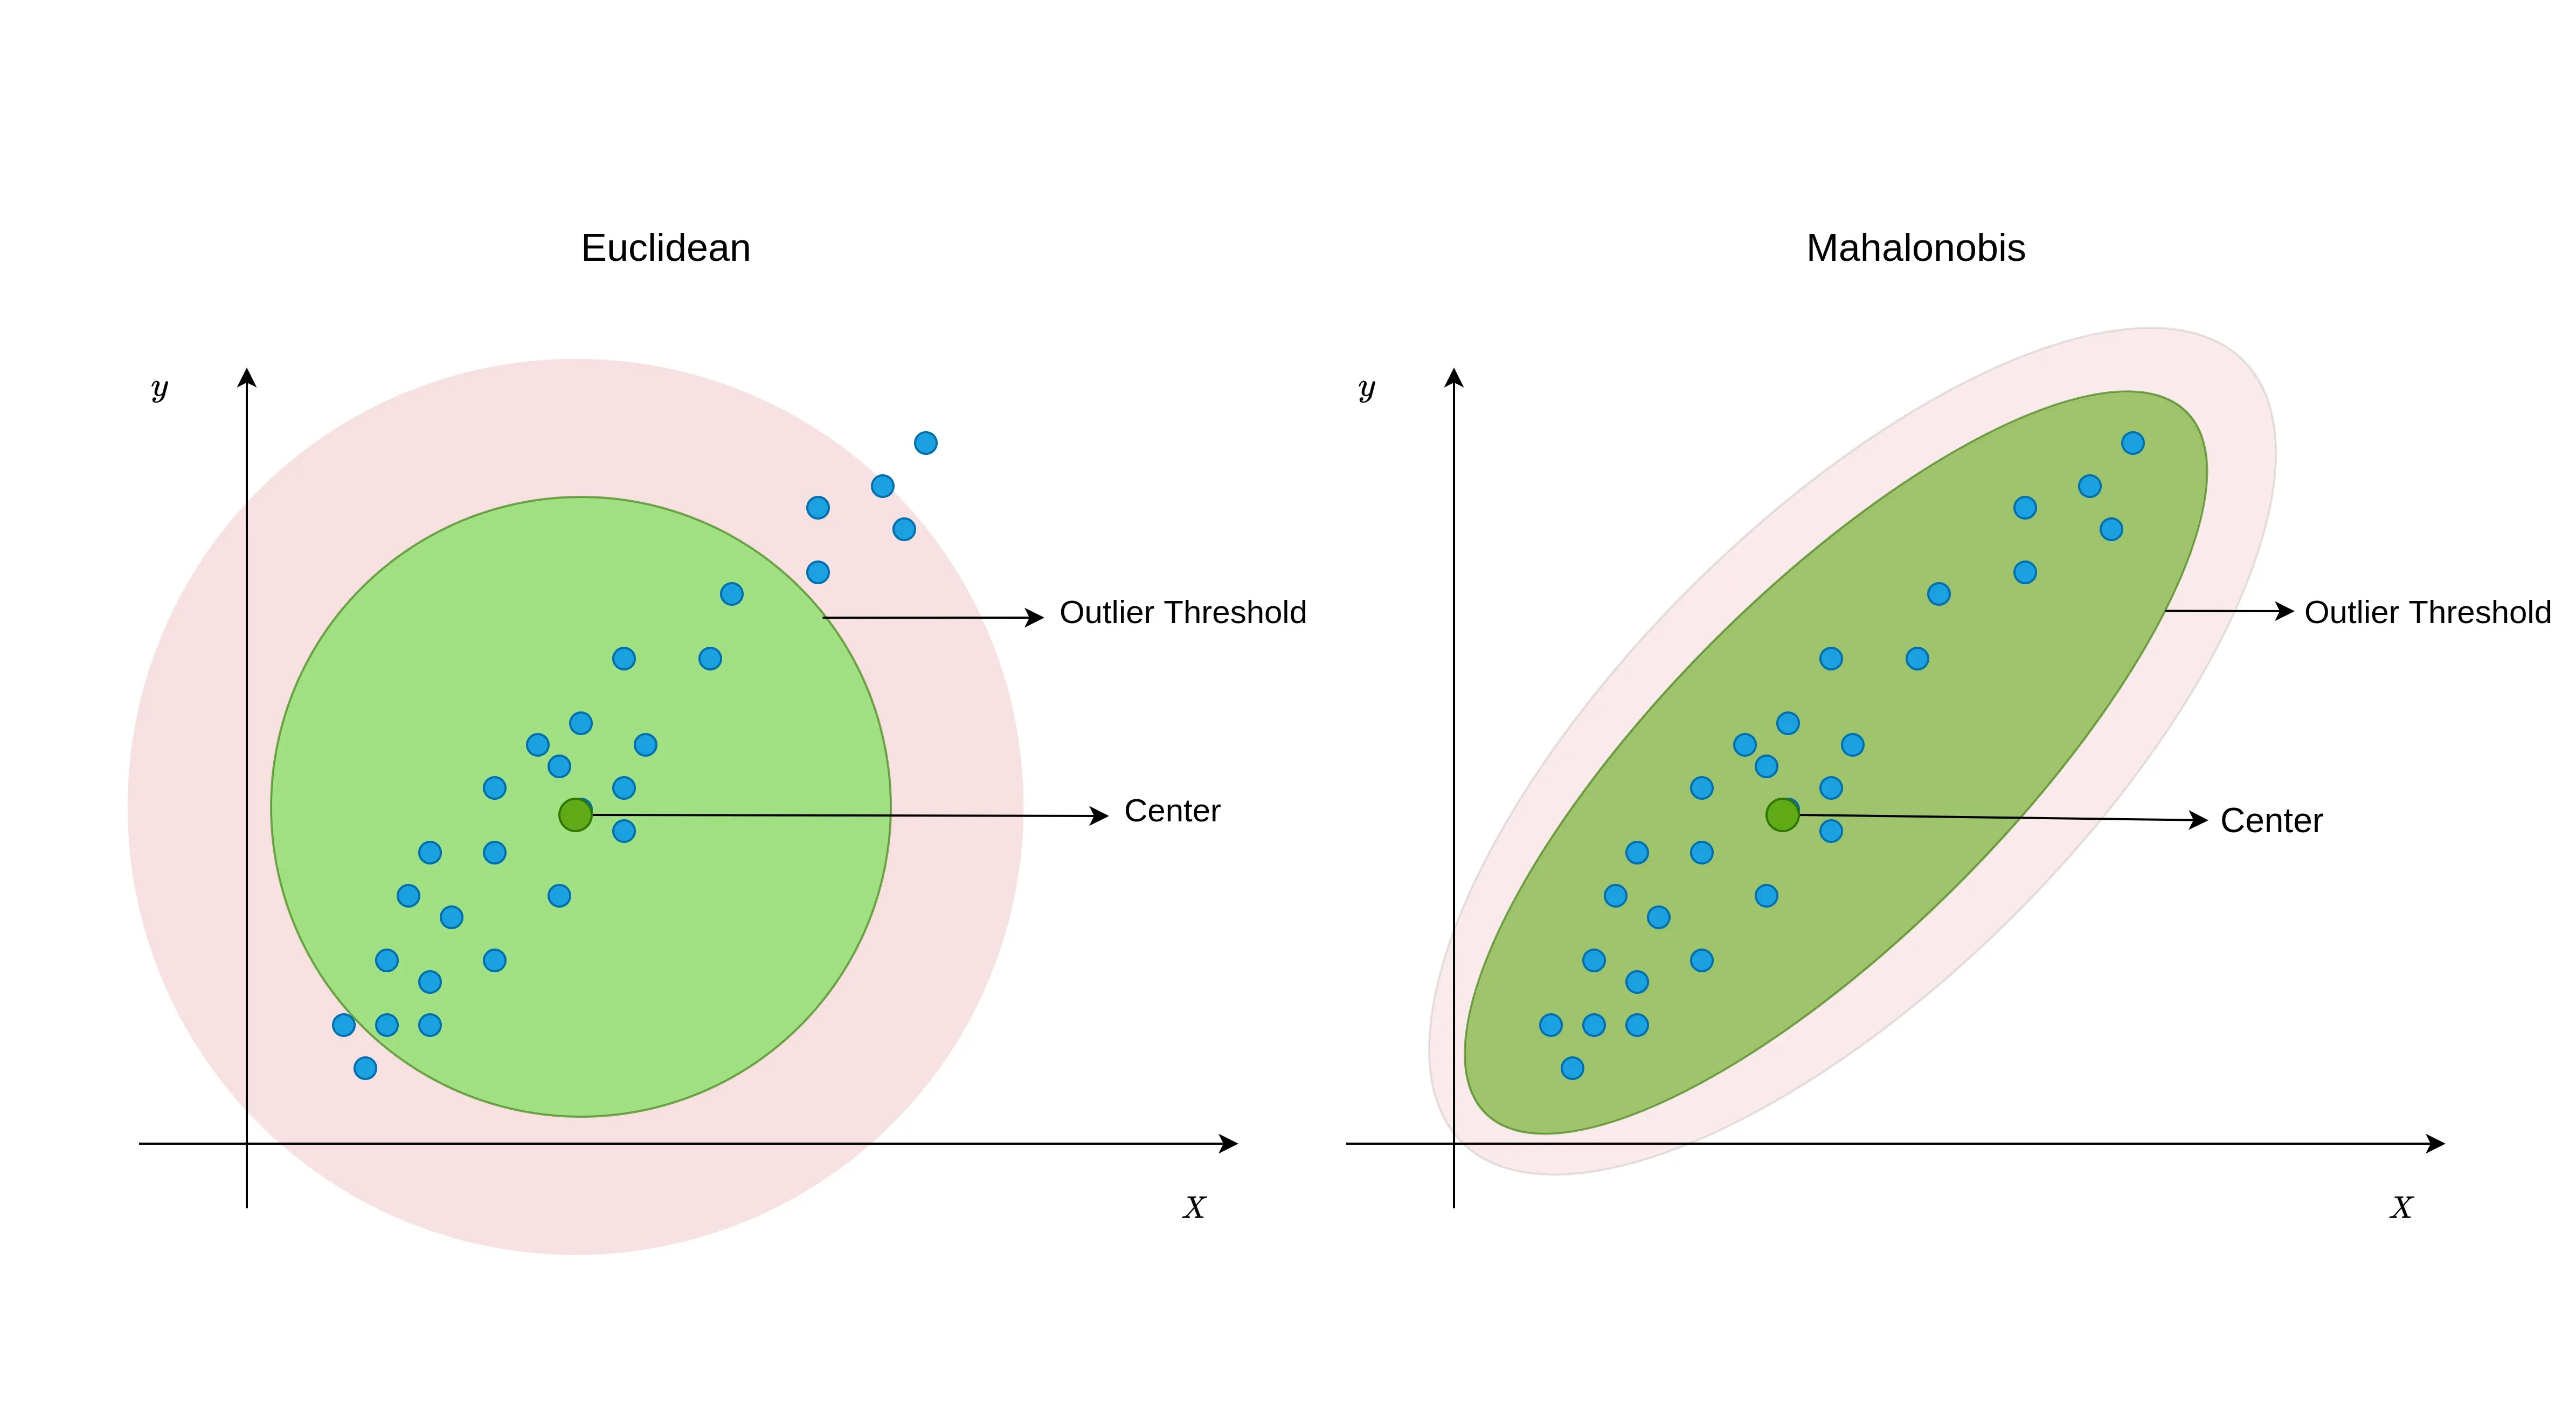
\includegraphics[width=0.9\linewidth]{Pictures/Optimizers/iSAM/Mahalanobis_Distance.png}
    \caption{Euclidean vs.\ Mahalanobis residual contours. \textit{Left:} isotropic (equal) weighting yields circular inlier regions. \textit{Right:} a covariance $\Sigma$ skews and scales the contours into an ellipse whose axes/tilt follow the noise correlations, whitening this with $\Sigma^{-1/2}$ maps this ellipse back to a circle.\textsuperscript{\cite{mahalanobis_distance_explained}}}
    \label{fig:mahalanobis-distance}
\end{figure}
\noindent
Mahalanobis distance is just ``error measured in the units of its noise'' (See Figure \ref{fig:mahalanobis-distance}). If a residual has high variance, it should be penalized less. If two components are correlated, they should not be treated as independent. That's what the covariance does. In the left plot (Euclidean), all directions are weighted equally so the inlier region is a circle. In the right plot (Mahalanobis), directions with low uncertainty are tighter and correlated axes tilt the ellipse. In SLAM cost function, each residual (process or measurement) is evaluated with its own covariance. Small reliable noises count more, whilst large noisy ones count less. When two parts of a measurement drift together, their error isn't along x or y alone, it's along some tilted direction. Mahalanobis tilts the ``penalty shape'' to match that direction. Penalties are smaller along noisy directions and larger where the sensor data is precise.
\\ \\
Equation \eqref{eq:optimizer-iSAM-delta-theta-star-mahalanobis-form} is a sum of Mahalanobis residuals (process terms use $\Lambda_i$, measurement terms use $\Gamma_k$). To turn that into one clean least squares system, first step is to ``whiten'' each residual so its noise is unit, for scalars divide by the standard deviation, for vectors apply the covariance's square root inverse to the residual and its Jacobians $\Sigma^{-1}$. After whitening, all errors are ordinary Euclidean ones, so the covariance symbols can be dropped, stack the Jacobians into one big sparse matrix $A$, stack the prediction errors into $b$, and solve the standard least squares problem \eqref{eq:optimizer-iSAM-delta-theta-star}.
\begin{equation}
    \Delta\theta^\star = \arg\min_{\Delta\theta}\; \|A\Delta\theta - b\|^2
    \label{eq:optimizer-iSAM-delta-theta-star}
\end{equation}
Here, $\theta$ stacks all unknowns (robot poses $x$ and landmarks $l$), $A$ is the single large, sparse (whitened) measurement Jacobian formed by stacking the block Jacobians $F, G, H,$ and $J$ from the linearized motion and measurement models, and $b$ is the stacked prediction error vector that collects the current odometry errors $a$ and measurement errors $c$ with a consistent sign convention. Intuitively, $A$ describes how residuals change for small state perturbations, $b$ encodes the present mismatch between predictions and measurements, and solving equation (\ref{eq:optimizer-iSAM-delta-theta-star}) yields the best local correction $\Delta\theta^\star$ used to update the estimate.
\\ \\
In the linearized setting, the optimal increment $\Delta\theta^\star$ is found by setting the gradient of the least squares objective to zero. This yields the normal equations according to iSAM paper \cite{iSAM_paper}:
$$
    A^{T}A\Delta\theta = A^{T}b
$$
Solving this system is typically performed using a numerically stable square root method (QR/Cholesky) rather than forming an explicit inverse. This gives the optimal correction $\Delta\theta^\star$. The state estimate is then updated as follows:
$$
    \theta \leftarrow \theta + \Delta\theta^\star
$$



\subsubsection{Incremental QR for fast updates (iSAM)}
The linearized SLAM subproblem is solved by least squares. Solving the normal equations $(A^\top A)\Delta\theta = A^\top b$ with Cholesky can be fast but very unstable and ill conditioned as the problem grows (it squares the condition number and increases fill in). iSAM avoids this by working directly with the whitened Jacobian $A$ using QR factorization, and by updating that factorization incrementally when new factors arrive.
\\ \\
Batch square root form (QR on the Jacobian) can be shown in iSAM paper \cite{iSAM_paper} to be of form:

$$
    A \;=\; Q
    \begin{bmatrix}
    R\\[2pt]
    0
    \end{bmatrix},
    \qquad Q^\top Q = I,
    \qquad R \text{: upper triangular}
$$
$$
    \begin{bmatrix}
    d\\ e
    \end{bmatrix}
    \;=\;
    Q^\top b
$$
$$
    \|A\Delta\theta - b\|^2
    \;=\;
    \|R\Delta\theta - d\|^2 + \|e\|^2
$$

\noindent
The iSAM paper \cite{iSAM_paper} shows that after QR the equation is:
$$
    A\Delta\theta - b \;=\;
    \begin{bmatrix} R \\ 0 \end{bmatrix}\Delta\theta -
    \begin{bmatrix} d \\ e \end{bmatrix},
    \quad\Rightarrow\quad
    \|A\Delta\theta - b\|^2 = \|R\Delta\theta - d\|^2 + \|e\|^2.
$$
\noindent
Put simply, once QR factorization is performed, the error splits into two parts. To make the total error as small as possible, set the first term to zero and solve:
\begin{equation}
    R\Delta\theta^\star = d
    \label{eq:optimizer-iSAM-fast-solution}
\end{equation}

\noindent
leaving $\|e\|^2$ as the (minimal) residual norm. If $R$ has full rank, this linearized system has one singular unique solution $\Delta\theta^\star$.
\\ \\
In iSAM the matrix $R$ is upper triangular, so equation (\ref{eq:optimizer-iSAM-fast-solution}) is solved by back substitution (no matrix inverse). This gives a fast, numerically stable way to compute the correction and update the state $\theta \leftarrow \theta + \Delta\theta^\star$ without heavy compute.



\subsubsection{What is R? The square root information matrix}
At the end of QR, the triangular factor $R$ satisfies the following form:
$$
R^\top R \;=\; A^\top A .
$$
This means $A^\top A$ (the information matrix obtained by linearization) is represented by the ``square root'' $R$. Working with $R$ keeps all the curvature of the problem but in a form that is easier to use and numerically safer because $R$ is upper triangular, so computations reduce to cheap substitution methods instead of expensive matrix inverses. Uncertainty can also be extracted directly from $R$. The state covariance is given by:
$$
\Sigma \;=\; (A^\top A)^{-1} \;=\; (R^\top R)^{-1},
$$
A dense inverse is never built. In reality, when entries of the uncertainty $\Sigma$ are needed, solve small triangular systems with $R^\top$ and $R$, and read only the pose blocks and the pose to landmark blocks of interest. Since $R$ is sparse and triangular, this is fast and stable, and it avoids forming $A^\top A$. (See \ref{sssec:iSAM-data-association} \nameref{sssec:iSAM-data-association})



\subsubsection{Matrix Factorization for building QR (Givens rotations)}
Here \emph{Givens rotations} is used to build an upper triangular factor $R$ from the (whitened) Jacobian $A$ by zeroing entries below the diagonal, one at a time. This yields a QR factorization without forming $A^\top A$ and without explicitly storing $Q$.
\\ \\
A Givens rotation is a $2\times 2$ orthogonal transform applied to two rows (or two columns) to annihilate one chosen entry. Givens rotation matrix is defined as:
\begin{equation}
    G(\varphi) =
    \begin{bmatrix}
        \cos\varphi & \sin\varphi \\
        -\sin\varphi & \cos\varphi
    \end{bmatrix}
    \label{eq:optimizer-iSAM-givens-rotation}
\end{equation}
Start at the leftmost non zero column of the $A$ matrix and sweep to the right, one column at a time. In each column, pick two rows, \textit{``k''} (the current pivot row) and \textit{``i''} (a row below it), and apply the small ``rotate and combine'' equation (\ref{eq:optimizer-iSAM-givens-rotation}) so the entry under the diagonal in that column becomes zero. Only those two rows are mixed, the new row \textit{``k''} becomes a bit of the old row \textit{``k''} plus a bit of row \textit{``i''}, and the new row \textit{``i''} becomes a bit of the old row \textit{``i''} minus a bit of row \textit{``k''}. Repeat down the column until all subdiagonal entries are gone, then move to the next column on the right. (see Figure \ref{fig:givens-rotation} down bellow for a visual of one Givens step)
\\ \\
As the algorithm sweeps the columns of $A$, the matrix is transformed into the upper triangular form, this is $R$, and the full $Q$ doesn't need to be formed to get to the result. Apply the same row rotations to $b$ as you eliminate entries so the right hand side stays consistent. After the initial factorization of $A$ matrix, new measurements don't require rebuilding $A$. Later it is shown that new whitened rows can be appended beneath the current $R$, then a short sequence of row rotations re-triangularizes $R$. In other words, updates operate directly on $R$ and $b$, and $A$ is bypassed for incremental steps.
\begin{figure}[H]
    \centering
    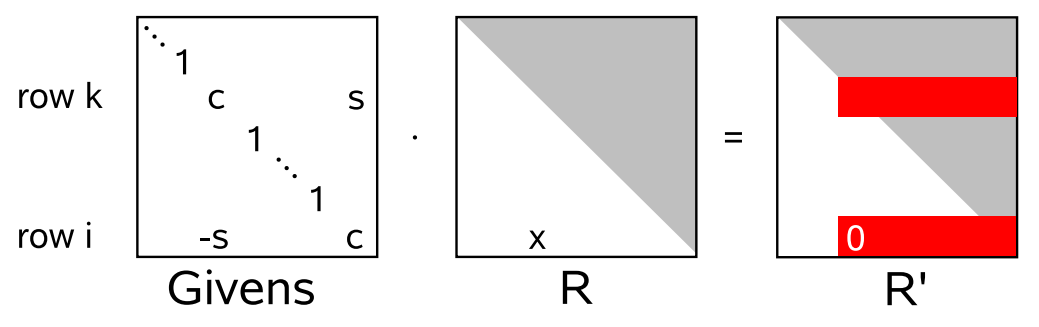
\includegraphics[width=0.9\linewidth]{Pictures/Optimizers/iSAM/Givens_Rotations.png}
    \caption{One Givens step in QR. The entry marked ``x'' is eliminated by rotating two rows, only the entries shown in red are modified, and the exact pattern depends on sparsity. Repeating this column wise (left to right) turns the matrix into an upper triangular $R$. Apply the same rotation to the $b$ vector to keep the least squares system consistent.\textsuperscript{\cite{iSAM_paper}}}
    \label{fig:givens-rotation}
\end{figure}
\noindent
In order to make $R$ upper triangular, $\varphi$ value must be chosen precisely to zero out a single sub diagonal entry in preliminary matrix, either be it $A$ matrix on batch step or $R$ matrix on iterative steps. The rotation angle $\varphi$ is computed from the two entries in the current column, the pivot $x=a_{kk}$ and the subdiagonal $y=a_{ik}$.
$$
    \begin{aligned}
        r=\sqrt{x^2+y^2}=\sqrt{a_{kk}^2+a_{ik}^2} \\
        c=\cos\varphi=\frac{x}{r}=\frac{a_{kk}}{r} \\
        s=\sin\varphi=\frac{y}{r}=\frac{a_{ik}}{r} 
    \end{aligned}
$$
Solving for $\varphi$ gives the following answer, where $\alpha = x = a_{kk}$ and $\beta = y = a_{ik}$:
\begin{equation}
    (\cos\varphi,\ \sin\varphi)=
    \begin{cases}
    (1,\,0), & \text{if }\beta=0,\\[6pt]
    \left(-\dfrac{\alpha}{\beta}\,\dfrac{1}{\sqrt{1+(\alpha/\beta)^2}},\ \dfrac{1}{\sqrt{1+(\alpha/\beta)^2}}\right), & \text{if }|\beta|>|\alpha|,\\[10pt]
    \left(\dfrac{1}{\sqrt{1+(\beta/\alpha)^2}},\ -\dfrac{\beta}{\alpha}\,\dfrac{1}{\sqrt{1+(\beta/\alpha)^2}}\right), & \text{otherwise.}
    \end{cases}
    \qquad\text{with }\ \alpha:=a_{kk},\ \beta:=a_{ik}.
    \label{eq:optimizer-iSAM-givens-rotation-find-phi}
\end{equation}
These coefficients in equation \eqref{eq:optimizer-iSAM-givens-rotation-find-phi} give the same rotation as \eqref{eq:optimizer-iSAM-givens-rotation}. 

Givens rotations guarantee that the $(i,k)$ entry of the working matrix becomes zero, and they preserve lengths. First the two numbers $[x,\,y]^\top$ are rotated. When embedded in the full matrix, the same rotation is applied to the affected parts of the two rows and to the matching entries of $b$. In practice, embed $G_{(i,k)}(\varphi)$ so it acts only on rows $k$ and $i$, and apply the same rotation to $b$ to keep the least squares system consistent.



\subsubsection{Incremental Updating}
\begin{figure}[H]
    \centering
    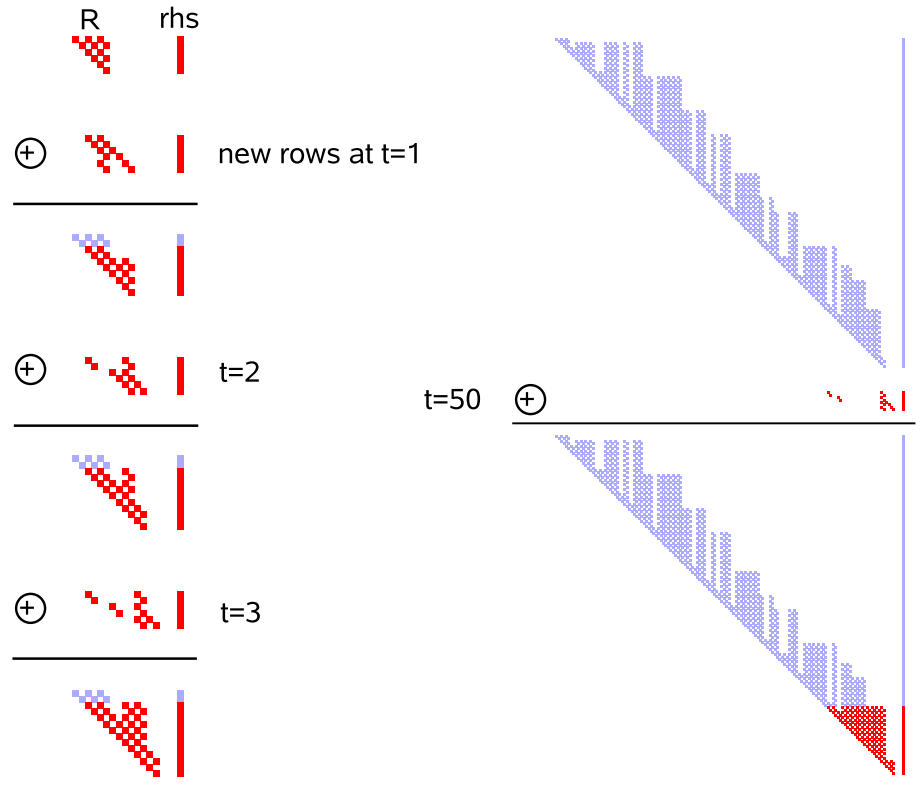
\includegraphics[width=0.5\linewidth]{Pictures/Optimizers/iSAM/R_Matrix_Update_Step.png}
    \caption{Incremental update of the factored system. A new whitened row $w^\top$ and RHS (Right Hand Side) entry $\gamma$ are appended beneath the current $R$ and $d$. A short sequence of Givens rotations restores the upper triangular form, yielding updated $R'$ and $d'$. Unchanged entries are shown in light color, only a small stencil is touched each step, so update cost stays bounded.\textsuperscript{\cite{iSAM_paper}}}
    \label{fig:R-matrix-update-step}
\end{figure}
\noindent
After the initial QR factorization, maintain the solution in ``square root'' form, an upper triangular matrix $R$ and a transformed right hand side $d$. Here, $R$ is the triangular factor that satisfies $R^\top R = A^\top A$ (the Gauss Newton information), and $d$ is the top part of $Q^\top b$. When a new measurement arrives, first whiten it (divide by its standard deviation or apply the square root information of its covariance) so it has unit variance. The whitened measurement contributes a new row $w^\top$ to the Jacobian and a new scalar $\gamma$ to the RHS (Right Hand Side). Notice that $A$ is NOT rebuild. Instead, append $w^\top$ under the current $R$, and $\gamma$ under the current $d$, which produces a system that is ``almost'' triangular but has one non triangular row at the bottom.
$$
    R' = \begin{bmatrix} R\\ w^\top \end{bmatrix},\qquad
    d' = \begin{bmatrix} d\\ \gamma \end{bmatrix}
$$
Next, re-triangularize locally with Givens rotations \eqref{eq:optimizer-iSAM-givens-rotation}. Only touching the columns where the new whitened Jacobian row $w^\top$ has nonzeros (i.e, the variables that this new factor actually connects to, such as a pose $x_i$ or a landmark $l_j$). Starting from the leftmost such column, each rotation mixes the current pivot row with the new bottom row to kill one sub diagonal entry. Repeat the process until the entire bottom row is zero and the matrix is upper triangular again. The equation would look something like this:
$$
    \begin{bmatrix} R\\ w^\top \end{bmatrix}
    \ \xrightarrow{\ \text{Givens rotation on affected columns}\ }\ 
    \begin{bmatrix} R'\\ 0 \end{bmatrix}
$$
While the matrix is rotates, apply the same rotations to the right hand side so that the least squares system stays consistent. Here $d$ is the transformed RHS (Right Hand Side) before the update and $\gamma$ is the new whitened RHS entry that pairs with $w^\top$. After the rotations, the top block becomes the updated RHS $d'$ used for solving, and the final bottom entry becomes a small leftover error $e_{\text{new}}$ that adds to the total residual. 
$$
    \begin{bmatrix} d\\ \gamma \end{bmatrix}
    \ \xrightarrow{\ \text{same rotations}\ }\ 
    \begin{bmatrix} d'\\ e_{\text{new}} \end{bmatrix}
$$
Intuitively, the new row $w^\top$ is ``folded up'' into the triangular structure by a short chain of 2x2 rotations that only touch the connected variables, everything else is left alone. Then get the correction by a fast back substitution on the updated matrix $R'$ and vector $d'$:
$$
    R'\Delta\theta^\star = d'
$$



\subsubsection{Loop Closure}
\begin{figure}[H]
    \centering
    % ---------- Left column ----------
    \begin{minipage}[t]{0.48\linewidth}
        \vspace{0pt}
        % Top-left (image 1)
        \begin{subfigure}[t]{\linewidth}
            \centering
            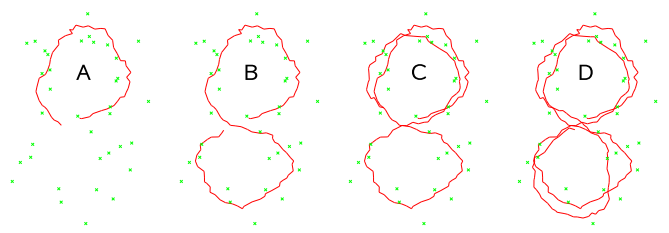
\includegraphics[width=\linewidth,height=0.47\textheight,keepaspectratio]{Pictures/Optimizers/iSAM/Variable_Reordering1.png}
            \caption{Simulated double 8 loop at key loop closure moments.\textsuperscript{\cite{iSAM_paper}}}\label{fig:l-top}
        \end{subfigure}\vspace{4pt}

        % Bottom-left row: (2) and (3) side-by-side
        \begin{subfigure}[t]{0.49\linewidth}
            \centering
            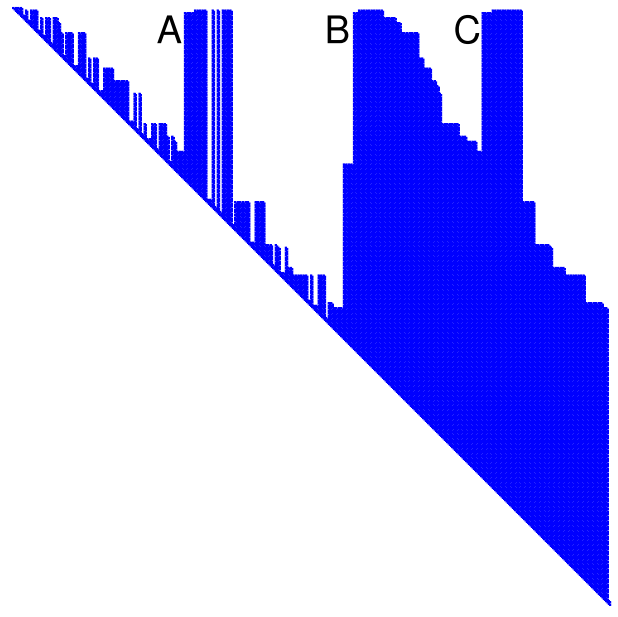
\includegraphics[width=\linewidth,height=0.20\textheight,keepaspectratio]{Pictures/Optimizers/iSAM/Variable_Reordering2.png}
            \caption{Upper triangular factor $R$ after several closures shows fill-in.\textsuperscript{\cite{iSAM_paper}}}\label{fig:l-bot-left}
        \end{subfigure}\hfill
        \begin{subfigure}[t]{0.49\linewidth}
            \centering
            
\includegraphics[width=\linewidth,height=0.20\textheight,keepaspectratio]{Pictures/Optimizers/iSAM/Variable_Reordering3.png}
            \caption{The same $R$ after variable reordering (COLAMD) becomes sparser again.\textsuperscript{\cite{iSAM_paper}}}\label{fig:l-bot-right}
        \end{subfigure}
    \end{minipage}\hfill
    % ---------- Right column ----------
    \begin{minipage}[t]{0.49\linewidth}
        \vspace{0pt}
        \begin{subfigure}[t]{\linewidth}
            \centering
            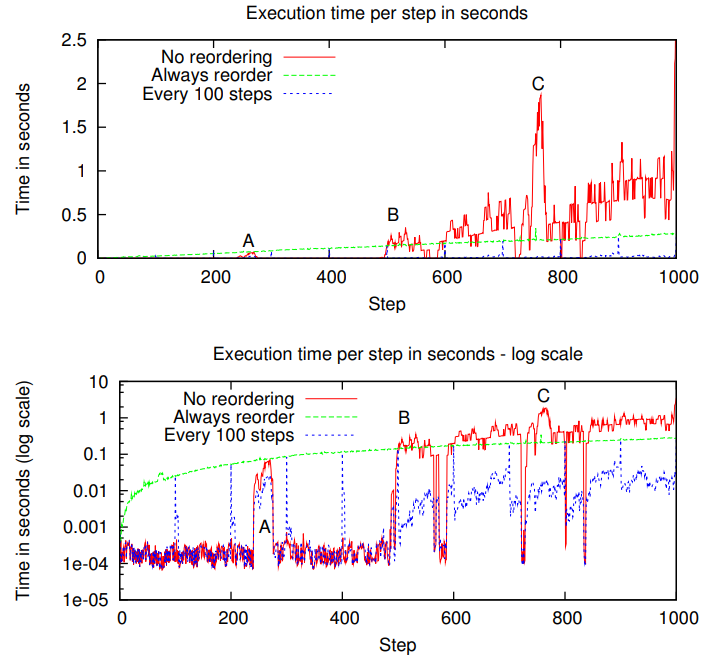
\includegraphics[width=\linewidth,height=0.98\textheight,keepaspectratio]{Pictures/Optimizers/iSAM/Variable_Reordering4.png}
            \caption{Per step execution time for three strategies. A: no reordering, B: reorder every step, C: reorder every 100 steps, shown in linear (top) and log (bottom) scale. Periodic reordering (C) limits spikes and keeps runtime predictable between loop closures.\textsuperscript{\cite{iSAM_paper}}}\label{fig:r-full}
        \end{subfigure}
    \end{minipage}

    \caption{Effect of loop closures and variable reordering (iSAM).\textsuperscript{\cite{iSAM_paper}}}
    \label{fig:variable-reordering}
\end{figure}
\noindent
Loop closures tie together far-apart parts of the trajectory (and landmarks), which makes previously separate columns interact. In QR terms this creates fill-in, R gets extra non zeros, so updates, back substitution, and selected covariance queries get slower and memory grows. This can be fixed by variable reordering. The goal is to pick a new elimination order that preserves sparsity. In practice run a heuristic like COLAMD (Column Approximate Minimum Degree) (often the block version for pose/landmark blocks) on the Jacobian's sparsity matrix $A$, then do batch factorization on the whole $A$ matrix using rotations \eqref{eq:optimizer-iSAM-givens-rotation} with that order \cite{iSAM_paper}. Reordering costs time because the factor must be rebuilt with a new permutation, but it pays back by making subsequent updates cheap again.
\\ \\
Because reordering is expensive, it is not done at every step. Instead, reordering is performed periodically every N steps (eks, 50 - 200) so the cost stays predictable. In marine AUV and ASV runs this keeps compute bounded. Between reorders incremental updates are fast and local. After a loop closure, one spike occurs (reorder + refactor), then the system returns to low latency. Practical tips when doing this step is to keep poses as blocks (block COLAMD) to reduce fill-in, align reordering with planned relinearization passes, and monitor simple stats (nonzeros in R, update time) to decide when N is too small (wasting time reordering) or too large (letting fill in snowball).  



\subsubsection{Re-Linearization}
Re-linearization keeps the local model valid. The QR and update methods assume the system is locally linear around the current estimate, but with angles, three dimensional motion, and nonlinear sensor data, that approximation drifts as the robot moves. If it is not refreshed, increments grow, the optimizer biases the map, and loop closures can fail. The remedy is to re-linearize and recompute Jacobians at the current state for the factors that matter. Doing this for every factor at every step is too expensive, so in practice new factors are always linearized, and older ones are refreshed only when needed.
\\ \\
In iSAM the practical schedule is to run incremental updates between maintenance cycles, then perform a full re-linearization every N steps. Between cycles, old factors are not re-linearized, new factors are whitened and inserted, and $R$ is updated incrementally. At the cycle boundary after N steps, the entire problem is re-linearized at the current estimate, the full Jacobian $A$ is rebuilt conceptually, variables are reordered with COLAMD to restore sparsity, and the system is refactored using equation \eqref{eq:optimizer-iSAM-givens-rotation} to obtain a fresh triangular $R$. For this reason variable reordering is usually grouped with batch re-linearization at the same N step.
\\ \\
$N$ must be chosen carefully, by balancing freshness vs compute. If N is too large, the linearization point drifts far from reality, Jacobians no longer match the true geometry, corrections become biased, loop closures pull hard, and the map can warp (a classic ``stale linearization'' issue). If $N$ is too small, the system stops often to re-linearize and refactor, wasting CPU and power, and reducing real-time throughput.



\subsubsection{Data Association from R}\label{sssec:iSAM-data-association}
For data association, Mahalanobis based approach is often used instead of plain nearest neighbour Approach. Nearest neighbour measures raw Euclidean distance and ignores sensor noise and correlations. Mahalanobis measures the innovation in the units of its uncertainty, so noisy directions count less, precise directions count more, and correlated components are handled correctly (See Figure \ref{fig:mahalanobis-distance}). For a candidate match between current pose $x_i$ and landmark $l_j$, form the innovation $\nu_k$ and score:
$$
    d_k^2=\nu_k^\top\,\Xi_k^{-1}\,\nu_k,\qquad
    \Xi_k=J_k\,\Sigma\,J_k^\top+\Gamma_k
$$
\noindent
where $J_k=[\,H^{x_i}\ \ H^{l_j}\,]$ is the linearized measurement Jacobian, $\Gamma_k$ is the sensor noise, and $\Sigma$ is the state covariance. 
\\ \\
This type of data association often uses gating with a chi-square test. The test keeps matches that are within $d_k^2\le \chi^2_{m,\alpha}$ (right dimension $m$, chosen confidence $\alpha$). From the survivors, pick the ``minimum cost'' one (or solve a global assignment using $d_{ij}^2$ as the cost matrix if several features compete). One thing to note about this approach is that the full dense $\Sigma=(R^\top R)^{-1}$ is not required for data association, only the local covariances influenced by the measurement. These covariances can be extracted directly from the square root information matrix $R$. Pose blocks and pose to landmark blocks are available online as well. Landmark terms on the other hand are either a approximate fast conservative estimate or computed exactly on demand. This keeps the association real-time for the most part.
Here are the partitioned forms.
Full state covariance (poses vs. landmarks):
$$
    \Sigma \;=\;
    \begin{bmatrix}
    \Sigma_{xx} & \Sigma_{xL}\\[4pt]
    \Sigma_{Lx} & \Sigma_{LL}
    \end{bmatrix}
$$
\noindent
where $\Sigma_{xx}$ is pose to pose, $\Sigma_{LL}$ is landmark to landmark, and $\Sigma_{xL}=\Sigma_{Lx}^\top$ is pose to landmark.
\\ \\
The $2\times2$ submatrix needed for a single candidate $(x_i,l_j)$:
$$
\Sigma_{\{x_i,l_j\}} \;=\;
\begin{bmatrix}
\Sigma_{x_i x_i} & \Sigma_{x_i l_j}\\[4pt]
\Sigma_{l_j x_i} & \Sigma_{l_j l_j}
\end{bmatrix}
$$
\noindent
\textbf{Fast marginals from the square root factor (online/live)} 
\\ \noindent
In iSAM paper \cite{iSAM_paper}, they propose keeping the current pose last in the ordering. Then the covariances needed for association, the pose variance $\Sigma_{x_i x_i}$ and the pose to landmark cross terms $\Sigma_{x_i l_j}$ come straight from the square root factor $R$ with two small triangular solves:
$$
    R^\top Y = B,\qquad R X = Y
$$
where $B=\begin{bmatrix}0\\ I_{d_x}\end{bmatrix}$ simply selects the last pose block of size $d_x$. Because $R$ is upper triangular and $B$ is zero above the last block, the forward solve gives:
$$
Y=\big[\,0,\ldots,0,\ R_{ii}^{-1}\,\big]^\top
$$
This $Y$ preliminary matrix is the clue, where only $d_x$ back substitutions are needed to get full $X$ vector. Reading the result $X$ yields, in one pass:
$$
\Sigma_{x_i x_i} \;\; \text{(bottom–right block of } \Sigma)\qquad
\Sigma_{l_j x_i}=\Sigma_{x_i l_j}^\top \;\; \text{for connected } l_j
$$
Intuitively ``solve up'' then ``solve down'' on $R$ for the last pose, and get exactly the columns of $\Sigma=(R^\top R)^{-1}$ that matter for gating in data association. This can be done every step without forming any dense inverses, only using $R$ square root information matrix iteratively. (See Figure \ref{fig:substitution-foward-backwards})
\begin{figure}[H]
  \centering
  \begin{subfigure}[t]{0.49\linewidth}
    \centering
    
\includegraphics[width=\linewidth]{Pictures/Optimizers/iSAM/Substitution_Forward.png}
    \caption{$R^\top Y = B$ (forward substitution). Sweep ``down'' the matrix to form $Y$ from a selector $B$ that picks the last pose block.}
    \label{fig:left}
  \end{subfigure}\hfill
  \begin{subfigure}[t]{0.49\linewidth}
    \centering
    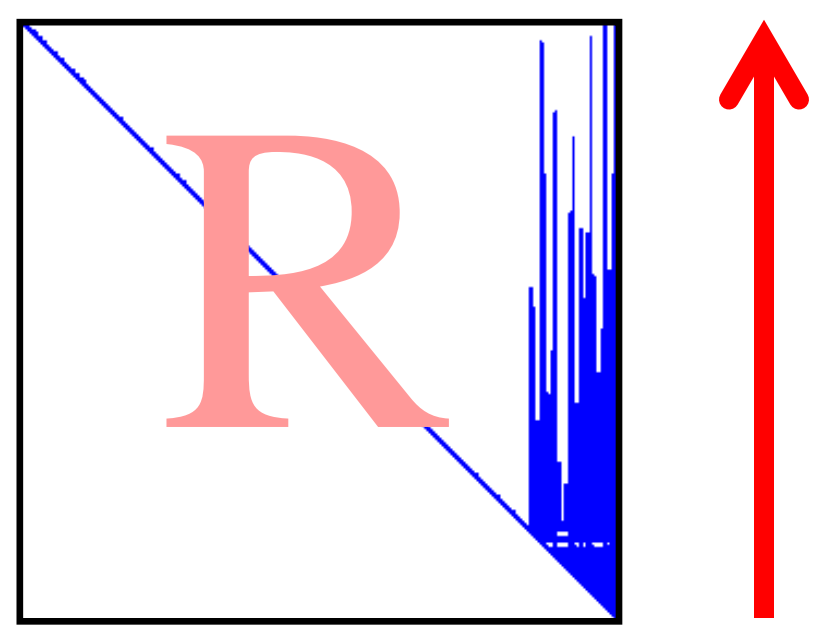
\includegraphics[width=\linewidth]{Pictures/Optimizers/iSAM/Substitution_Downwards.png}
    \caption{$R X = Y$ (back substitution). Sweep ``up'' the matrix to obtain the desired columns $X=\Sigma_{:\,,x_i}$ (pose and pose to landmark).}
    \label{fig:right}
  \end{subfigure}
  \caption{Grab the needed covariances in two quick steps: first solve ``down'' with $R^\top$, then solve ``up'' with $R$. Only touch entries near the last pose block, so each update stays fast and cheap.\textsuperscript{\cite{iSAM_paper}}}
  \label{fig:substitution-foward-backwards}
\end{figure}
\noindent
\textbf{Conservative landmark covariances (online/live)} 
\\ \noindent
Exact landmark landmark blocks $\Sigma_{jj}$ (or old pose to landmark $\Sigma_{(i-n)j}$) are expensive to extract at every step. Therefore in iSAM paper \cite{iSAM_paper} they propose using a safe, conservative bound built from the current pose covariance and the measurement noise via the linearized back projection:
$$
    \tilde\Sigma_{jj}
    \;=\;
    \bar J\,
    \begin{bmatrix}
    \Sigma_{ii} & 0\\[2pt]
    0 & \Gamma
    \end{bmatrix}
    \bar J^\top
$$
where $\bar J$ is the Jacobian of the local inverse measurement model, $\Sigma_{ii}$ is the current pose covariance, and $\Gamma$ is the measurement noise. This upper bounds landmark uncertainty (never over confident), is fast, and works well for online Mahalanobis gating. As more measurements of a landmark arrive, this bound typically tightens.
\\ \\
An important caveat to mention is that the true $\Gamma$ (measurement noise) is usually unknown. The iSAM recipe is to choose $\Gamma$ conservatively so the algorithms doesn't get overly confident. That keeps things safe but can make the gate too tight, causing the data association to reject more matches than it should. Later, a more reliable way to approximate $\Gamma$ from measurement characteristics is described. It avoids overconfidence and uses cues such as sonar range and resolution and landmark confidence, so the gate is realistic and not risky.
\\ \\
\textbf{Exact landmark covariances (on demand)} 
\\ \noindent
When accuracy is needed (eks: on risky loop closure, conflicting hypotheses), Data Association can recover exact $\Sigma_{jj}$ and $\Sigma_{(i-n)j}$ without forming the full dense inverse information matrix $\Sigma=(A^{T}A)^{-1}=(R^{T}R)^{-1}$. Because the covariance is the inverse of the information matrix:
$$
    \Sigma=(R^\top R)^{-1}, \qquad R^\top R\,\Sigma = I
$$
Needed entries can be extracted without forming the full inverse by solving for two triangular matrixes:
$$
R^\top Y = I, \qquad R \Sigma = Y
$$
The solve uses only the ``nonzero'' entries of $R$, so computation touches only the parts that matter, not the whole matrix. iSAM walks backwards along those non zero links and gives us exactly the covariance numbers $\sigma_{ij}$ Data Association ask for. If $R$ is mostly banded, this is near linear time. This exact method should only be used when its really needed (eks: a few $\Sigma_{jj}$ blocks to check on a loop closure). It's slower than the conservative shortcut, but still much faster than inverting the whole matrix.
\\ \\
\textbf{Alternative way to finding $\Gamma$} 
\\ \noindent
There's another angle. Instead of being very conservative with $\Gamma$ measurement noise. Uncertainty used in Data Association should reflect the sensor, for example a sonar for scanning the sea floor. With sonar the measurement noise can grow with range, and the transducer resolution can set per axis variances $N(0, \Sigma_{sonar})$. The landmark detection can also contribute its own uncertainty $N(0, \Sigma_{landmark})$. In practice these are combined to form the prediction uncertainty for the residual that is scored. In that case the effective covariance is:
$$
    \Gamma = Var(h(x, l)) = \Sigma_{sonar} + \Sigma_{landmark}
$$
This can be more informative than a one size fits all setting. However, this approach requires care. If the noise terms are too confident, the data association gate becomes too tight, matches become brittle, and the system can become unstable. Nevertheless, it often yields more accurate maps and a better estimate of the robot's track.



\subsubsection{Algorithm}
At each time step absorb new information, linearize around the current estimate, solve a small least squares, and update. Periodically refresh linearization and variable order. Concretely:
\begin{enumerate}
    \item \textbf{Add factors (whiten first):} take the new odometry/measurements and add them to the graph. ``Whiten”'' them so every residual has unit noise (as described before \eqref{eq:optimizer-iSAM-delta-theta-star}).

    \item \textbf{Linearize at the current guess \(\theta\):} turn the nonlinear motion/measurement models into local linear ones using the Jacobians in
    \eqref{eq:optimizer-iSAM-linearized-odometry} and \eqref{eq:optimizer-iSAM-linearized-measurement}. This gives the summed Mahalanobis cost \eqref{eq:optimizer-iSAM-delta-theta-star-mahalanobis-form}, which after whitening becomes one least squares problem \eqref{eq:optimizer-iSAM-delta-theta-star}.

    \item \textbf{Keep a triangular system up to date (QR):} append the new (whitened) rows and apply a few Givens rotations \eqref{eq:optimizer-iSAM-givens-rotation} so the matrix stays upper triangular $R$. Update the right hand side $b$ vector the same way (see ``Incremental Updating'').

    \item \textbf{Solve for the small change:} because $R$ is triangular, solve
    \eqref{eq:optimizer-iSAM-fast-solution} by back substitution (fast) to get the correction .

    \item \textbf{Update the estimate:} replace the old state with the improved one,
    $\theta \leftarrow \theta + \Delta\theta^\star$.

    \item \textbf{Every \(N\) steps (maintenance):} refresh accuracy by re-linearizing all factors at the new $\theta$, reorder variables (eks: COLAMD algorithm) to keep things sparse, and refactor with Givens \eqref{eq:optimizer-iSAM-givens-rotation} to get a clean $R$.

    \item \textbf{Data Association update:} read the needed covariances from $R$ (pose and pose to landmark live, landmark blocks conservative or exact on demand) and run Mahalanobis gating in Data Association for next matches.
\end{enumerate}



\subsubsection{Limitations}
iSAM is fast between updates but has practical downsides. They come from the ``data structure'', not the underlying SLAM algorithm. iSAM keeps a single, global square root information matrix $R$ (from $A^\top A$) and does periodic maintenance (reordering + re-linearization). This makes updates simple, but couples cost to global structure and variable ordering instead of just local changes.
\begin{itemize}
    \item \textbf{Latency spikes at maintenance:} Periodic global variable reordering and re-linearization trigger stalls (especially after loop closures), since $R$ must be refactored end to end.

    \item \textbf{Fill in growth between reorders:} Incremental QR on a fixed order accumulates fill in in $R$, touching more entries per update and increasing time/memory step by step.

    \item \textbf{All or nothing re-linearization:} iSAM typically refreshes many factors at maintenance even if most variables barely moved, wasting Jacobian recomputations.

    \item \textbf{Global refactor on ordering changes:} Any change to elimination order implies a large refactor of the global $R$, regardless of how small the new information is.

    \item \textbf{Broad marginal queries are costly:} Last pose and nearby cross terms can be pulled quickly from $R$, but wide $\Sigma$ blocks (eks: many landmarks or older poses) require multiple triangular solves and can be costly.

    \item \textbf{Schedule sensitivity:} Choosing ``every $N$ steps'' for reorder/re-linearize is heuristic, too small wastes time, too large lets fill in and linearization error grow, causing jitter and warp in the map.

    \item \textbf{Numerical robustness vs simplicity:} Working with $A$ and $R$ avoids explicit $A^\top A$, but long incremental runs plus fill in can still hurt conditioning and stability if ordering lags.
\end{itemize}
\noindent
These limitations motivated \textbf{iSAM2}, which replaces the single monolithic $R$ that is very static, with a Bayes tree representation that is dynamic and updates only the affected parts. We address iSAM2 and how it mitigates the issues above in the next chapter.

 \clearpage
\subsection{iSAM2}
iSAM2 stuff here \clearpage
\subsection{GTSAM}
GTSAM stuff here \clearpage

 \clearpage

% Refrences
\newpage
\printbibliography

\end{document}
% Document (STSTOPART) ==================================================

